%%%%%%%%%%%%%%%%%%%%%%%%%%%%%%%%%%%%%%%%%%%%%%%%%%%%%%%%%%%%%%%%%%%%%%%%%%%%%%%%
%2345678901234567890123456789012345678901234567890123456789012345678901234567890
%        1         2         3         4         5         6         7         8

\documentclass[11pt]{article}
\usepackage{fullpage}
\usepackage{color}
\usepackage{multirow}
\usepackage{float}
\usepackage{graphicx}
\usepackage{caption}
\usepackage{subcaption}
\usepackage{booktabs}
\usepackage{amsmath}
\usepackage{amsfonts}
\usepackage{algpseudocode}
\usepackage{algorithm, algorithmicx}
\usepackage{hyperref}



\usepackage{graphics} % for pdf, bitmapped graphics files
\usepackage{graphicx}

\title{
  Matrix Factorizations at Scale: a Comparison of Scientific Data Analytics in Spark and C+MPI Using Three Case Studies 
}

\author{Alex Gittens$^{1}$ \and Aditya Devarakonda$^{2}$ \and Evan Racah$^{3}$ \and Michael Ringenburg$^{4}$ \and  Lisa Gerhardt$^{3}$ \and Jey Kottaalam$^{5}$ \and Jialin Liu$^{3}$ \and Kristyn Maschhoff$^{4}$ \and Shane Canon$^{3}$ \and Jatin Chhugani$^{6}$ \and Pramod Sharma$^{4}$ \and Jiyan Yang$^{7}$ \and James Demmel$^{8}$ \and Jim Harrell$^{4}$ \and Venkat Krishnamurthy$^{4}$ \and Michael W. Mahoney$^{1}$ \and Prabhat$^{3}$% <-this % stops a space
\thanks{$^{1}$ICSI and Department of Statistics, UC Berkeley}
\thanks{$^{2}$EECS, UC Berkeley}
\thanks{$^{3}$NERSC, Lawrence Berkeley National Laboratory}
\thanks{$^{4}$Cray, Inc.}
}

\date{July 1, 2016}

\begin{document}
\maketitle

\begin{abstract}
%Data analysis has rapidly become an important part of scientific discovery. There exist many easy-to-use data analytics frameworks for domain scientists to use, however, they are well-suited for data-parallel tasks and record-based database-like transactions. In addition, scalability of these frameworks to large numbers of nodes has not been well-studied. 
We explore the trade-offs of performing linear algebra using Apache Spark, compared to traditional C and MPI implementations on HPC platforms. Spark is designed for data analytics on cluster computing platforms with access to local disks and is optimized for data-parallel and database-like tasks. We examine three widely-used and important matrix factorizations: NMF (for physical plausability), PCA (for its ubiquity) and CX (for data interpretability). We apply these methods to TB-sized problems in particle physics, climate modeling and bioimaging.  The data matrices are tall-and-skinny which enable the algorithms to map conveniently into Spark's data-parallel model. We perform scaling experiments on up to 1600 Cray XC40 nodes, describe the sources of slowdowns, and provide tuning guidance to successfully attain peak performance using Spark. 
\end{abstract}

\section{Introduction}
\label{sec:introduction}
Modern scientific progress relies upon experimental devices, observational instruments, and scientific simulations. These important modalities produce massive amounts of complex data: in High Energy Physics, the LHC project produces PBs of data every month; smaller-scale projects such as Daya Bay produce 100s of TBs over their lifetime. In Climate science, the worldwide community relies upon distributed access to the CMIP-5 archive, which is several PBs in size. In  Biosciences, each experiment can acquire 100GBs-TBs of data. In all cases, a considerable amount of effort is spend in data movement and data management issues, but the key step in gaining scientific insights is \emph{data analytics}. Several scientific domains are currently rate-limited by access to advanced (but convenient/user-friendly) parallel and scalable data analytics methods. 

Some of the most important classes of scientific data analytics methods rely on matrix algorithms. 
Matrices provide a convenient mathematical structure with which to model data arising in a broad range of applications: an $m \times n$ real-valued matrix $A$ provides a natural structure for encoding information about $m$ objects, each of which is described by $n$ features; alternatively, an $n \times n$ real-values matrix $A$ can be used to describe the correlations between all pairs of $n$ data points. 
Matrix factorizations are common in numerical analysis and scientific computing, where the emphasis is on running time, largely since they are used simply to enable the rapid solution of linear systems and related problems.
In statistical data analysis, however, matrix factorizations are typically used to obtain some form of lower-rank (and therefore simplified) approximation to the data matrix $A$ to enable better understanding the structure of the data~\cite{HMH00}.
In particular, rather than simply providing a mechanism for solving another problem quickly, the actual components making up a factorization are of prime concern.
Thus, it is of interest to understand how popular factorizations interact with other aspects of the large-scale data analysis pipeline.
%\textcolor{red}{Michael: I need 4-6 lines on matrix factorizations and why they are important}.

Along these lines, recent years have seen a tremendous amount of momentum behind Big Data software frameworks such as Hadoop/MapReduce~\cite{DG04} and Spark~\cite{SPARK_HOTC_10}. 
These frameworks have been developed for industrial applications and commodity datacenter hardware; and they provide high productivity computing interfaces for the broader data science community.  
Ideally, the scientific data analysis and high performance computing (HPC) communities would leverage the momentum behind Hadoop and Spark.
Unfortunately, the performance of such frameworks at scale on conventional HPC hardware has not been investigated extensively. 
For matrix factorizations in particular, and largely motivated by scientific computing, the research community has a distinguished track record in developing linear algebra libraries (ScaLAPACK, LAPACK, BLAS, PLASMA, MAGMA, etc.~\cite{lapack99,PlasmaMagma2009}). 
Our work takes on the important task of testing nontrivial linear algebra and matrix factorization computations in Spark for real-world, large-scale scientific data analysis applications, carefully comparing and contrasting its performance with C+MPI implementations on HPC hardware. 

The main contributions of this paper are as follows:
\begin{itemize}
\item{We develop parallel versions of three leading matrix factorizations (PCA, NMF, CX) in Spark and C+MPI; and we apply them to several TB-sized scientific datasets.}
\item{We conduct strong scaling tests on a XC40 system, and we test the scaling of Spark on up to 1600 nodes.}
\item{We characterize the performance gap between Spark and C+MPI for matrix factorizations, and we comment on current limitations in Spark for large scale scientific data analytics in HPC environments.}
\end{itemize}

The paper is structured as follows: Section \ref{sec:science} presents three science drivers from Particle Physics, Climate Science and BioImaging, and it motivates data analytics challenges at scale. Section \ref{sec:methods} presents the algorithms and implementation details of three matrix factorization methods. Section \ref{sec:setup} presents details of our HPC platform and Spark/C+MPI code configuration; and we then present results of our investigation in Section \ref{sec:results}. We conclude with observations on current Spark limitations in \ref{sec:lessons} and broader implications for linear algebra computations in Section \ref{sec:conclusions}. 

\section{Science Drivers and Data sets}
\label{sec:science}
\begin{figure*}
\centering
\begin{subfigure}[b]{0.32\textwidth}
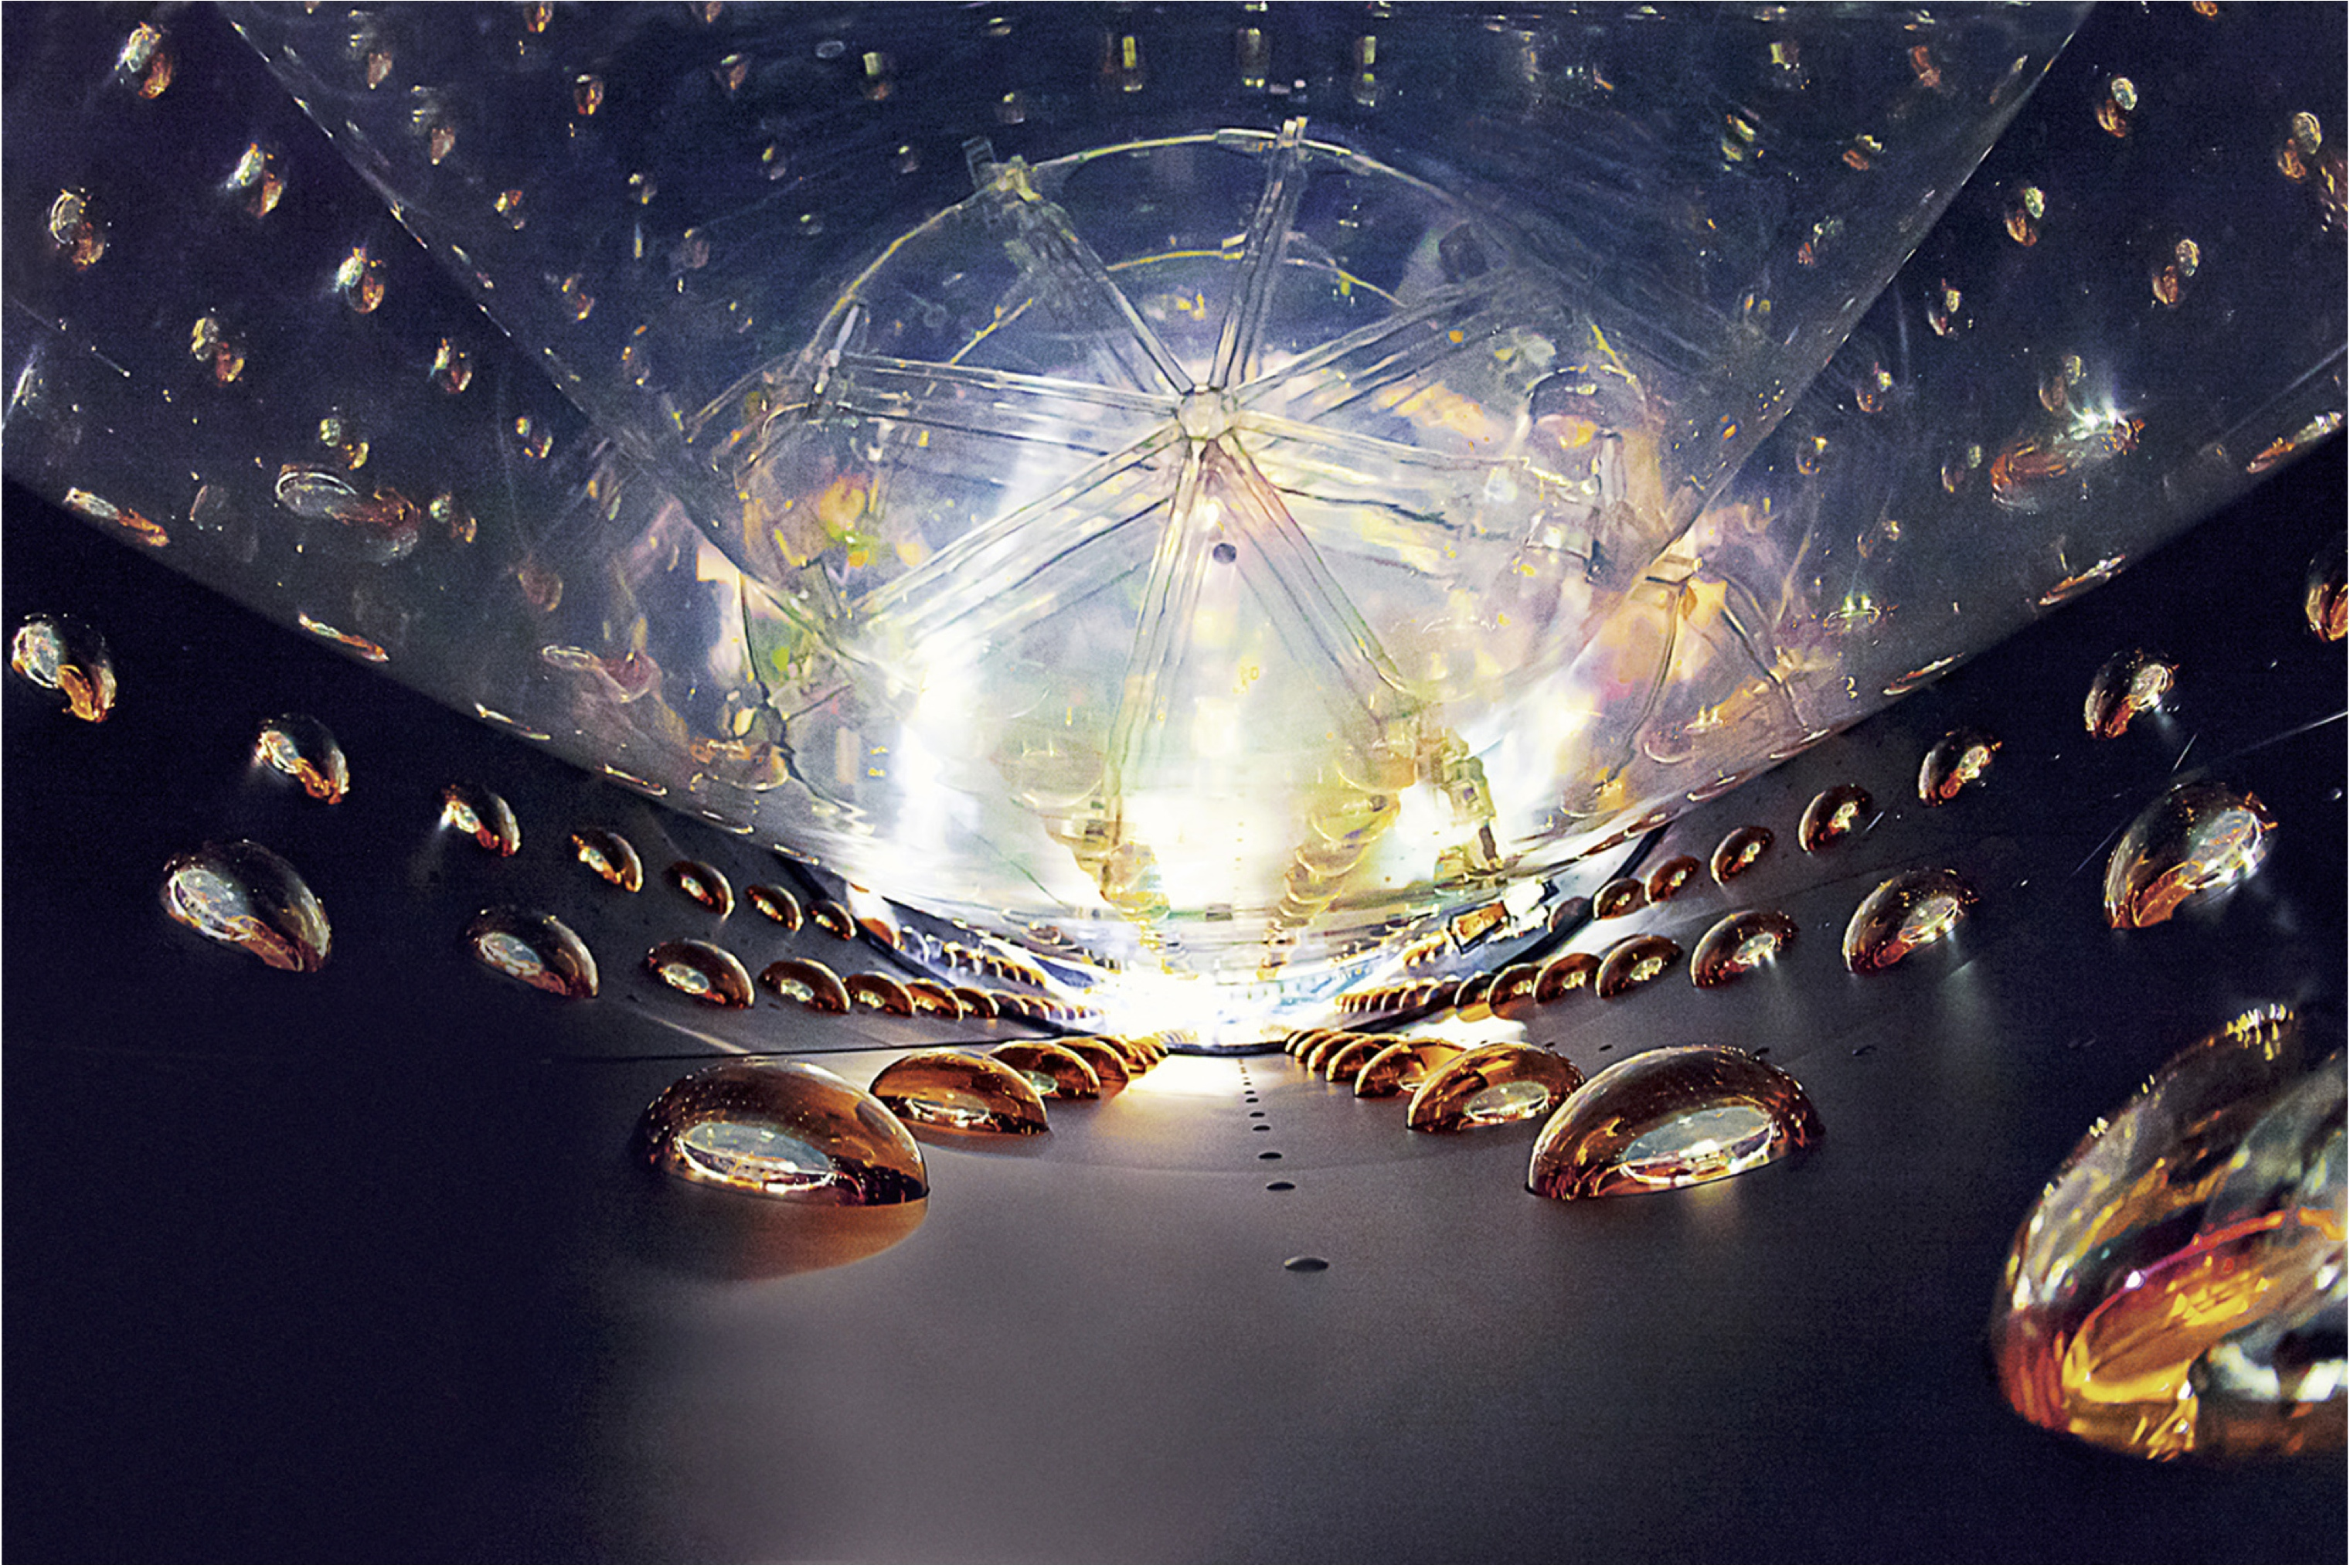
\includegraphics[width=\textwidth]{fig/dayabay.jpg}
\caption{Daya Bay Neutrino Experiment}
\label{fig:dayabay}
\end{subfigure}
\begin{subfigure}[b]{0.42\textwidth}
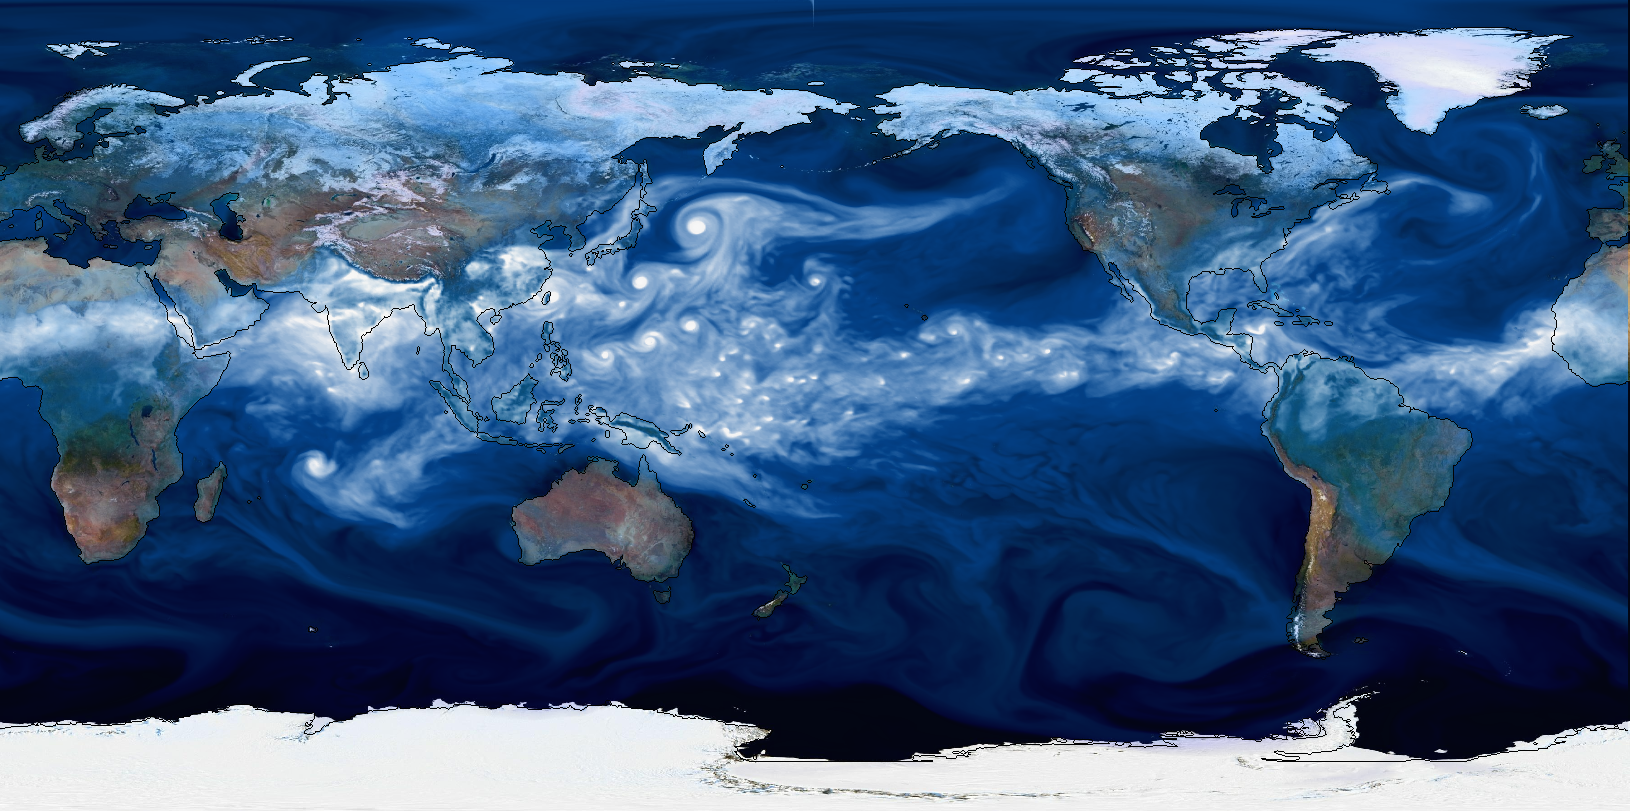
\includegraphics[width=\textwidth]{fig/climate.png}
\caption{CAM5 Simulation}
\label{fig:cam5}
\end{subfigure}
\begin{subfigure}[b]{0.22\textwidth}
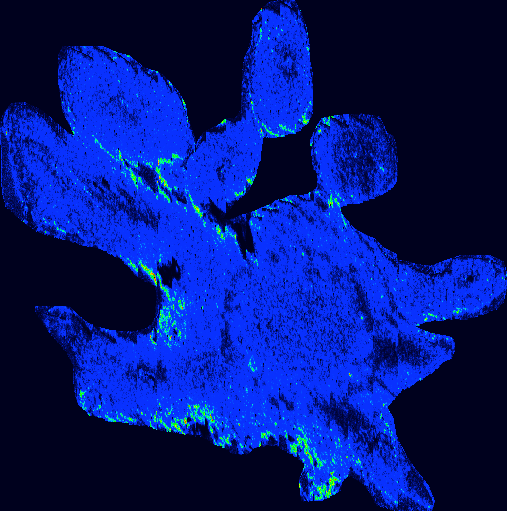
\includegraphics[width=\textwidth]{fig/mass-spec.png}
\caption{Mass-Spec Imaging}
\label{fig:mass-spec}
\end{subfigure}
\caption{Sources of various data sets used in this study}\label{fig:datasets}
\end{figure*}
In this study, we choose leading data sets from experimental, observational, and simulation sources, and we identify associated data analytics challenges. 
%We compare the performances of our MPI and Spark implementations of the low-rank decompositions on: a 1.6TB-sized sparse matrix obtained from the Daya Bay Neutrino Experiment for NMF decomposition;  a 2.2TB and 16TB-sized dense matrix of oceanic (reanalysis) and atmospheric (simulation) variables for PCA decomposition; and a 1TB-sized sparse matrix obtained via mass spectrometry imaging for  CX decomposition. All matrices were processed in double precision. 
The properties of these data sets are summarized in Table~\ref{table:datasets}.

\begin{table}[ht]
\centering
\caption{Summary of the matrices used in our study}
\label{table:datasets}
\begin{tabular}{p{2cm}lllll@{}}
\toprule
Science Area & Format/Files & Dimensions & Size  \\ \midrule
MSI      & Parquet/2880        &  $8,258,911 \times 131,048$          & 1.1TB  \\
Daya Bay & HDF5/1      &   $1,099,413,914 \times 192$         & 1.6TB \\
Ocean              & HDF5/1      &  $6,349,676 \times 46,715$          & 2.2TB \\
Atmosphere           & HDF5/1       & $26,542,080 \times 81,600$           & 16TB \\ \bottomrule
\end{tabular}
\end{table}



\paragraph{The Daya Bay Neutrino Experiment.}
The Daya Bay Neutrino Experiment (Figure \ref{fig:dayabay}) is situated on the southern coast of China. It detects antineutrinos produced by the Ling Ao and Daya Bay nuclear power plants and uses them to measure theta-13, a fundamental constant that helps describe the flavor oscillation of neutrinos. In 2012 the Daya Bay experiment measured this with unprecedented precision. This result was named one of the Science magazines top ten breakthroughs of 2012, and this measurement has since been refined considerably \cite{dayabay15}.

The Daya Bay Experiment consists of eight smaller detectors, each with 192 photomultiplier tubes that detect light generated by interaction of anti-neutrinos from the nearby nuclear reactors. Each detector records the total charge in each of the 192 photomultiplier tubes, as well as the time the charge was detected. For this analysis we used a data array comprised of the sum of the charge for every photomultiplier tube from each Daya Bay detector. This data is well suited to NMF analysis since accumulated charge will always be positive (with the exception of a few mis-calibrated values). The extracted data was stored as HDF5 files with 192 columns, one for each photomultiplier tube, and a different row for each discrete event in the detectors. The resulting data set is a sparse 1.6 TB matrix. The specific analytics problem that we tackle in this paper is that of finding characteristic patterns or signatures corresponding to various event types. Successfully ``segmenting'' and classifying a multiyear long timeseries into meaningful events can dramatically improve the productivity of scientists and enable them to focus on anomalies, which can in turn result in new physics results.

\paragraph{Climate Science.}
Climate scientists rely on HPC simulations to understand past, present and future climate regimes. Vast amounts of 3D data (corresponding to atmospheric and ocean processes) are readily available in the community. Traditionally, the lack of scalable analytics methods and tools has prevented the community from analyzing full 3D fields; typical analysis is thus performed only on 2D spatial averages or slices. The most widely used tool for extracting important patterns from the measurements of atmospheric and oceanic variables is the Empirical Orthogonal Function (EOF) technique. EOFs are popular because of their simplicity and their ability to reduce the dimensionality of large nonlinear, high-dimensional systems into fewer dimensions while preserving the most important patterns of variations in the measurements. Mathematically, EOFs are exactly PCA decompositions.

In this study, we consider the Climate Forecast System Reanalysis Product~\cite{saha:2010}. Global Ocean temperature data, spatially resolved at 360 x 720 x 41 (latitude x longitude x depth) and 6-hour temporal resolution is analyzed. The CFSR data set yields a dense 2.2TB matrix. We also process a CAM5 0.25-degree atmospheric humidity data set~\cite{wehner:2014} (Figure~\ref{fig:cam5}). The grid is 768 x 1158 x 30 (latitude x longitude x height) and data is stored every 3 hours. The CAM5 data set spans 28 years, and it yields a dense 16TB matrix. The specific analytics problem that we tackle is finding the principal causes of variability in large scale 3D fields. A better understanding of the dynamics of large-scale modes of variability in the ocean and atmosphere may be extracted from full 3D EOFs.

%We apply our PCA implementations to the analysis of ocean temperatures collected in 6 hours increments over a global  latitude-longitude-depth grid, extracted from the . Unfolding each 3D grid set of temperature measurements into a long vector and taking the vectors formed in this way to be columns of a matrix yields a dense 2.2TB matrix. Further, we also compute the EOFs of 28 years of measurements of atmospheric variable collected at 3 hours increments over a global 768-by-1152-by-30 latitude-longitude-height grid, \textcolor{red}{what is the provenance?}. Forming the matrix as in the case of the ocean temperatures yields a dense 16TB matrix. To the best of our knowledge, this is the first published work where climate fields of these sizes have been subjected to EOF analysis.
%Traditionally, EOFs have been calculated on two-dimensional slices of fields due to the difficulties climate scientists face when attempting to apply their usual computational tools to the immense amount of data present in the full 3D fields.· %The EOF modes extracted in this manner project the true complex 3D patterns involving multiple layers of the atmospher or ocean onto the considered slice. A better understanding of the dynamics of large-scale modes of variability in the ocean and atmosphere may be extracted from full 3D EOFs.
\paragraph{Mass-Spectrometry Imaging.}
Mass spectrometry measures ions derived from the molecules present in a biological sample. Spectra of the ions are acquired at each location (pixel) of a sample, allowing for the collection of spatially resolved mass spectra. This mode of analysis is known as \textit{mass spectrometry imaging (MSI)}. The addition of \textit{ion-mobility separation (IMS)} to MSI adds another dimension, drift time.  The combination of IMS with MSI is finding increasing applications in the study of disease diagnostics, plant engineering, and microbial interactions. Unfortunately, the scale of MSI data and complexity of analysis presents a significant challenge to scientists: a single 2D-image may be many gigabytes and comparison of multiple images is beyond the processing capabilities available to many scientists. The addition of IMS exacerbates these problems. 

We analyze one of the largest (1TB sized) mass-spec imaging data sets in the field, obtained from a sample of the plant {\it Lewis Dalisay Peltatum} (Figure \ref{fig:mass-spec}). The MSI measurements are formed into a sparse matrix whose rows and columns correspond to pixel and ($\tau$, $m/z$) values of ions, respectively. Here $\tau$ denotes drift time and $m/z$ is the mass-to-charge ratio. The sheer size of this data set has previously made complex analytics intractable. CX decompositions allow for the possibility of identifying small numbers of columns (ions) in the original data that reliably explain a large portion of the variation in the data.




\section{Methods}
\label{sec:methods}

\subsection{Matrix Factorizations}

Given an $m \times n$ data matrix $A$, low-rank matrix factorization methods aim to find two or more smaller matrices such that their product is a good approximation to $A$.
That is, they aim to find matrices $Y$ and $Z$ such that
\begin{equation*}
 \label{eqn:apprx}
    \underset{m\times n}{A} \approx \underset{m\times k}{Y} \times \underset{k\times n}{Z}. 
\end{equation*}
Low-rank matrix factorization methods are important tools in linear algebra and numerical analysis, and they find use in a variety of scientific fields and scientific computing.

Depending on the application, various low-rank factorization techniques are of interest. Popular choices include the singular value decomposition~\cite{GVL96}, principal component analysis~\cite{pcaBook}, rank-revealing QR factorization~\cite{GE96}, nonnegative matrix factorization (NMF) ~\cite{NMFalg}, and CUR/CX decompositions~\cite{CUR_PNAS}.

In this work, we consider the PCA decomposition due to its ubiquity and the NMF and CX decompositions due to their usefulness in scalable and interpretable data analysis. In the remainder of the section, we briefly describe these decompositions and the algorithms we used in our implementations.
% For an arbitrary matrix $A$, denote by $\a_i$ its $i$-th row, $\a^j$ its $j$-th column and $\a_{ij}$ its $(i,j)$-th element. 
Throughout, we assume the data matrix $A$ has size $m \times n$ and rank $r$, with $r \ll n \ll m.$ We denote its $i$-th row and $j$-th column respectively with $a_i$ and $a^j$, and we denote its $(i,j)$-th element with $a_{ij}.$

\subsubsection{PCA} 
The singular value decomposition (SVD) is the most fundamental low-rank matrix factorization because it provides the best low-rank matrix approximation with respect to any unitarily invariant matrix norm.
In particular, for any target rank $k \leq r$, the SVD provides the minimizer of the optimization problem
\begin{equation}
 \label{eqn:obj}
  \min_{\text{rank}(\tilde A) = k} \| A - \tilde A \|_F,
\end{equation}
where the Frobenius norm $\| \cdot \|_F$ is defined as $\|X\|_F^2 =
\sum_{i=1}^m \sum_{j=1}^n X_{ij}^2 $. Specifically, the solution
to~\eqref{eqn:obj} is given by the truncated SVD, i.e., $A_k = U_k \Sigma_k
V_k^T$, where the columns of $U_k$ and $V_k$ are the top $k$ {\it left and right singular vectors}, respectively, and $\Sigma_k$ is a 
diagonal matrix containing the corresponding top $k$ {\it singular values}.

Principal component analysis (PCA) and SVD are closely related: the PCA decomposition of $A$ is defined as the SVD of the matrix formed by centering each column of $A$ (i.e., removing the mean of each column).
%PCA aims to convert the original features into a set of linearly uncorrelated variables called {\it principal components}.
%The first principal component is defined to be the direction along which the highest variance possible among the data points is attained, and each succeeding principal component in turn has the largest variance possible subject to the constraint that it is orthogonal to the preceding principal components.
%When low-rank methods are appropriate, the number of principal components needed to preserve most of the information in $A$ is far less than the number of original features. 

\begin{algorithm}[tb]
    \caption{\textsc{PCA} Algorithm}
    \label{alg:pca}
    \begin{algorithmic}[1]
      \Require $A \in \mathbb{R}^{m\times n}$, rank parameter $k \leq \textrm{rank}(A).$
      \Ensure $U_k \Sigma_k V_k^T = \textsc{PCA}(A, k).$
      \State Let $(V_k, \_) = \textsc{IRAM}(\textsc{MultiplyGramian}(A, \cdot), k).$
      \State Let $Y = \textsc{Multiply}(A, V_k).$
      \State Compute $(U_k, \Sigma_k, \_) = \textsc{SVD}(Y).$
    \end{algorithmic}
  \end{algorithm}
  
Direct algorithms for computing the PCA decomposition scale as $\mathcal{O}(mn^2)$, so are not feasible for the scale of the problems we consider. Instead, we use the iterative algorithm presented in Algorithm~\ref{alg:pca}: in step 1, a series of distributed matrix-vector products against $A^T A$  (\textsc{MultiplyGramian}) are used to extract $V_k$ by applying the implicitly restarted Arnoldi method (\textsc{IRAM})~\cite{lehoucq1996deflation}, then in step 2 a distributed matrix-matrix product followed by a collect is used to bring $AV_k$ to the driver. Step 3 occurs on the driver, and computes a final SVD on $AV_k$ to extract the top left singular vectors $U_k$ and the corresponding eigenvalues $\Sigma_k.$ Here QR and SVD compute the ``thin'' versions of the QR and SVD decompositions~\cite{GVL96}. (Algorithm~\ref{alg:pca} calls \textsc{MultiplyGramian}, which is summarized in Algorithm~\ref{alg:gram}).

  \begin{algorithm}[tb]
    \caption{{\sc MultiplyGramian} Algorithm}
    \label{alg:gram}
    \begin{algorithmic}[1]
      \Require $A \in \mathbb{R}^{m\times n}$, $B \in \mathbb{R}^{n\times k}$.
      \Ensure $X = A^T A B$.
      \State Initialize $X = 0$.
      \For{each row $a$ in $A$}
          \State $X \gets X + a a^T B$.
      \EndFor
    \end{algorithmic}
\end{algorithm}
  
\subsubsection{NMF}
Although the PCA provides a mathematically optimal low-rank decomposition in the sense of~\eqref{eqn:obj}, in some scientific applications retaining sparseness and interpretability is as important as explaining variability. The nonnegative matrix factorization (NMF) provides an interpretable low-rank matrix decomposition when the columns of $A$ are nonnegative and can be viewed as additive superpositions of a small number of positive factors~\cite{gillis2014and}. NMF has found applications, among other places, in medical imaging~\cite{lee2001nmf}, facial recognition~\cite{guillamet2002non}, chemometrics~\cite{Paatero199723}, hyperspectral imaging~\cite{gillis2015hierarchical}, and astronomy~\cite{pauca2006nonnegative}.

\begin{algorithm}[tb]
    \caption{\textsc{NMF} Algorithm}
    \label{alg:nmf}
    \begin{algorithmic}[1]
      \Require $A \in \mathbb{R}^{m\times n}$ with $A \geq 0$, rank parameter $k \leq \textrm{rank}(A).$
      \Ensure $W H \approx A$ with $W,H \geq 0$
      \State Let $(\_, R) = \textsc{TSQR}(A).$
      \State Let $(\mathcal{K}, H) = \textsc{Xray}(R, k).$
      \State Let $W = A(:, \mathcal{K}).$
    \end{algorithmic}
  \end{algorithm}
  
The optimization problem solved by NMF is
\begin{equation}
\min_{W,H \geq 0} \|A - WH\|_F,
\end{equation}
where $W \in \mathbb{R}^{m \times k}$ and $H \in \mathbb{R}^{k \times n}$ are entry-wise nonnegative matrices. Typical approaches attempt to solve this non-convex problem by using block coordinate optimizations that require multiple passes over $A$~\cite{kim2014algorithms}. We adopt the one-pass algorithm of~\cite{benson2014scalable}. This approach makes the assumption that $W$ can be formed by {\it selecting} columns from $A$. In this setting, the columns of $A$ constituting $W$ as well as the corresponding $H$ can be computed directly from the (much smaller) $R$ factor in a thin QR factorization of $A$. More details are given in Algorithm~\ref{alg:nmf}: in step 1, a one pass distributed tall-skinny QR (\textsc{TSQR}) factorization~\cite{demmel2012communication} is used to compute the $R$ factor of $A$; in step 2, which occurs on the driver, the \textsc{Xray} algorithm of~\cite{kumar2013fast} is applied to $R$ to simultaneously compute $H$ and the column indices $\mathcal{K}$ of $W$ in $A$. Finally, $W$ can be explicitly computed once $\mathcal{K}$ is known.

\subsubsection{CX}
CX decompositions are
low-rank matrix decompositions that are expressed in terms of a small number of columns/rows, i.e, actual data elements.  As such, they have been used in scientific applications where coupling analytical techniques with domain knowledge is at a premium, including
genetics~\cite{Paschou07b}, astronomy~\cite{Yip14-AJ}, and mass spectrometry imaging~\cite{YRPMB15}. To find a CX decomposition, we seek matrices $C$ and $X$ such that the approximation error $\|A-CX\|_F$ is small and $C$ is an $m\times k$ matrix comprising of $k$
actual columns of $A$ and $X$ is a $k \times n$ matrix.

% Let $V_k$ contain the top $k$ right singular vectors of $A$. Given a target rank parameter $k$, for $i=1,\ldots,n$, the $i$-th leverage score is defined as
%   \begin{equation}
%    \label{eqn:lev}
%     \ell_i = \sum_{j=1}^k v_{ij}^2.
%   \end{equation}
% These scores quantify the amount of ``leverage'' each column of $A$ exerts on the best rank-$k$ approximation to $A$. If, for $i=1,\ldots,n$, we define the {\it normalized leverage scores} as
%   \begin{equation}
%   \label{eqn:nlev}
%     p_i = \frac{\ell_i}{\sum_{j=1}^n \ell_j},
%   \end{equation}
% where $\ell_i$ is defined in~\eqref{eqn:lev}, and choose columns from $A$ according to those normalized leverage scores, then (by~\cite{DMM08,CUR_PNAS}) the selected columns are able to reconstruct the matrix $A$ nearly as well as $A_k$ does.

The randomized algorithm of~\cite{DMM08} generates a $C$ whose approximation error is, with high probability, within a multiplicative factor of $(1+\varepsilon)$ of the optimal error obtainable with a low-rank decomposition:
\[
\|A - CX\|_F \leq (1+ \varepsilon) \|A - A_k\|_F.
\]
This algorithm takes as input the (approximate or exact) \emph{leverage scores} of the columns of $A.$ The leverage score of the $j$-th column of $A$ is defined in terms of $V_k$, the matrix of top k right singular vectors:
  \begin{equation}
    \label{eqn:lev}
     \ell_i = \sum_{j=1}^k (V_k) _{ij}^2;
   \end{equation}
the leverage scores can be approximated using an approximation to $V_k.$ The CX algorithm uses those scores as a sampling distribution to select $k$ columns from $A$ to form $C$; once the matrix $C$ is determined, the optimal matrix $X$ that minimizes $\|A-CX\|_F$ can be computed accordingly; see~\cite{DMM08} for the details of this construction.

%  \begin{algorithm}[tb]
%    \caption{\textsc{CX} Decomposition}
%     \label{alg:cx}
%     \begin{algorithmic}[1]
%       \Require $A \in \mathbb{R}^{m\times n}$, rank parameter $k \leq \textrm{rank}(A)$, number of power iterations $q$.
%       \Ensure $C$.
%       \State Compute an approximation of the top-$k$ right singular vectors of $A$ denoted by $\tilde V_k$, using \textsc{RandomizedSVD} with $q$ power iterations.
%       \State Let $\ell_i = \sum_{j=1}^k \tilde v_{ij}^2$, where $\tilde v_{ij}^2$ is the $(i,j)$-th element of $\tilde V_k$, for $i = 1, \ldots, n$.·
%       \State Define $p_i = \ell_i / \sum_{j=1}^d \ell_j$ for $i=1,\ldots,n$.
%       \State Randomly sample $k$ columns from $A$ in i.i.d. trials, using the importance sampling distribution $\{p_i\}_{i=1}^n$ .
%       \end{algorithmic}
% \end{algorithm}

The computational cost of the CX decomposition is determined by the cost of computing $V_k$ exactly or approximately. To approximate $V_k$, we use the \textsc{RandomizedSVD} algorithm introduced in \cite{MRT06,MRT11}. We refer the readers to \cite{HMT09_SIREV,Mah-mat-rev_BOOK} for more details. Importantly, the algorithm runs in $\mathcal{O}(mn \log k)$ time and needs only a constant number of passes over the data matrix ($q$+1), where $q$ is an input in Algorithm~\ref{alg:cx}).  The \textsc{RandomizedSVD} algorithm comprises the first nine steps of Algorithm~\ref{alg:cx}. The running time cost for \textsc{RandomizedSVD} is dominated by a distributed matrix-matrix multiplication appearing in Steps 3 and 7 of Algorithm~\ref{alg:cx}. After Step 7, $Y$ is collected the remaining computations are carried out on the driver.

\begin{algorithm}[tb]
   \caption{{\sc CX} Algorithm}
    \label{alg:cx}
    \begin{algorithmic}[1]
      \Require $A \in \mathbb{R}^{m\times n}$, \
        number of power iterations $q \ge 1$, \
        target rank $k > 0$, slack $p \ge 0$, and let $\ell=k+p$.

      \Ensure $C$.

      \State Initialize $B \in \mathbb{R}^{n\times \ell}$ by sampling $B_{ij} \sim \mathcal{N}(0, 1)$.

      \For{$q$ times}
          \State $B \gets \Call{MultiplyGramian}{A, B}$
          \State $(B, \_) \gets \Call{QR}{B}$
      \EndFor

      \State Let $Q$ be the first $k$ columns of $B$.

      \State Let $Y = \Call{Multiply}{A, Q}$.

      \State Compute $(U, \Sigma, \tilde V^T) = \Call{SVD}{Y}$.

      \State Let $V = Q \tilde V$.

	  \State Let $\ell_i = \sum_{j=1}^k v_{ij}^2$ for $i = 1, \ldots, n$.
      
      \State Define $p_i = \ell_i / \sum_{j=1}^d \ell_j$ for $i=1,\ldots,n$.
      
      \State Randomly sample $k$ columns from $A$ in i.i.d. trials, using the importance sampling distribution $\{p_i\}_{i=1}^n$ .
      \end{algorithmic}
  \end{algorithm}



\section{Implementation}
\label{sec:implementation}

\subsection{Spark as a Data Analytics Platform} \textcolor{blue}

Spark is a parallel computing framework, built on the JVM, that adheres to the data parallelism model. A Spark cluster is composed of a driver process and a set of executor processes. The driver controls and schedules the work, which is turn handed off to the exectors. The basic unit of work in Spark is called a task. A single executor has many slots for running tasks and will run several concurrent tasks in the course of calculations; although it can be changed, by default one task is assigned to one core available to the executor. Each user-defined code that is to be calculated is called an application. When an application is submitted to the cluster, the driver analyses it and breaks it up into jobs. Each job represents an action on the dataset, such as counting the number of entries, returning dataset extries, or saving a dataset to a file. Jobs are further broken down into stages, which are collections of tasks each executing the same code on a different subset of data. Spark converts input data into a resilient distributed dataset or RDD. Each RDD is split into multiple partitions and a single task works on a single partition.

\subsection{Implementing Matrix Factorizations in Spark}

\subsection{Implementing Matrix Factorizations in C+MPI}
NMF, PCA and CX require linear algebra kernels that are widely available in libraries such as Intel MKL, Cray LibSci and arpack-ng. We make use of these libraries to perform linear algebra computations required for each matrix factorization. The data matrices are represented as 1D arrays of double-precision floating point numbers and are partitioned across multiple nodes. The matrix factorizations implemented and matrix shapes used require 1D-block partitioned layouts which enable us to use data parallel kernels such as matrix-vector products and TSQR. We predominately use MPI collectives for inter-processor communication and perform independent I/O using the Cray HDF5 parallel I/O library.  

\section{Experimental Setup}
\label{sec:setup}
\subsection{Cori}
All performance tests reported in this paper were conducted on the Cori system at NERSC. Cori Phase I is a Cray XC40 system with 1632 dual-socket compute nodes. Each node consists of two 2.3GHz 16-core Haswell processors and 128GB of DRAM. The Cray Aries high-speed interconnect is configured in a `dragonfly' topology. We utilize a Lustre scratch filesystem with 27PB of storage, and over 700 GB/s peak I/O performance. 

\subsection{Spark Configuration}
We use the Standalone Cluster Manager to run the Spark cluster. This is a collection of scripts that start the driver process and use ssh to start the executor processes on each node. Once the executors are started they communicate with the driver via akka-tcp. When an application is submitted to the Spark cluster a second java process is spawned by each executor that controls the computation for that application. Sometimes this second process will fail to start and executor does not participate in the calculation. The exact cause of this is not well known. Running Spark in an encapsulated Shifter image (see Section \ref{shiftersec}) reduces the rate of these failures, which suggests this could be due to a race condition in the code

\subsection{H5Spark: Loading HDF5 data natively into Spark}
The NMF and PCA data are both stored in HDF5, which is a hierarchical array model. Spark needs to read this data as one RDD object first before other data analytic jobs can continue. We used H5Spark~\cite{h5spark-cug16} to accomplish this. H5Spark provides a parallel I/O interface that efficiently loads TBs of data into the workers' memory and constructs a single RDD. A MPI-like independent I/O is performed in H5Spark to balance the workload. H5Spark partially relies on the Lustre file system striping to achieve the high bandwidth. We chose a Lustre configuration optimal for each dataset: we stored the NMF data on 72 OSTs and the PCA data on 140 OSTs, both with striping size of 1MBs. Currently, H5Spark's IO is independent of MPIIO.

\subsection{Shifter} \label{shiftersec}
Shifter is a framework that delivers docker-like functionality to HPC \cite{shifter}. It works by extracting images from native formats (such as a Docker image) and converting them to a common format that is optimally tuned for the HPC environment. On Cori at NERSC, users can pull down images directly from Docker or from other private registries and run this image on thousands of nodes simultaneously. This functionality is tied into the slurm batch system and requested images are automatically started at the beginning of jobs. Shifter allows users with a complicated software stack to easily install them in the environment of their choosing. It also offers considerable performance improvements because metadata operations can be more efficiently cached compared to a parallel file system and users can customize the shared library cache (ldconfig) settings to optimize access to their analysis libraries. In particular, shared library performance, which has long been a pain point on Cray machines, is dramatically improved.
Shifter provides a user-controlled option to create a writeable temporary space that is private to each node.  This has performance characteristics similar to a local disk which many Cray systems, such as Cori, lack.  However, this is created by mounting a writeable loop-back mounted file system which is backed by the parallel file system.

For this analysis we used two separate Shifter images. A generic “CCM” image which only contained SSH functionality (which is otherwise absent by default on Cray compute nodes) and a full “spark” image which contained version 1.5.1 of Spark  compiled with OpenBLAS \cite{openblas} and SSH. The Spark image is available on docker \cite{dockerspark}. 

\subsection{Spark Tuning Parameters}

Shifter provides a user-controlled option to create a writeable temporary space that is private to each node. This has performance characteristics similar to a local disk which many Cray systems, such as Cori, lack. This is created by mounting a writeable loop-back mounted file system which is backed by the parallel file system. This feature is very useful to frameworks like Spark that assume the presence of a local disk that can be used to store node local temporary files and spills. Metadata operations and small I/O transaction can  be more efficiently cached on the compute node since, unlike the Lustre scratch file system, it doesn't have to maintain coherency of this file system with other nodes. Most importantly, as the Spark cluster size is scaled up, this approach helps avoid additional pressure on the Lustre Metadata Servers which are the least scalable component of the file system. Since Spark opens and closes files many times, using the loop-back mounted file system as a writable cache can improve performance \cite{scalingspark16}.

We followed general Spark guidelines for Spark configuration values. The driver and executor memory were both set to 100 GB, a value chosen to maximize the memory available for data caching and shuffling while still leaving a buffer to hedge against running the nodes out of memory.  Generally we found that fetching an RDD from another node was detrimental to performance, so we turned off speculation (a function that restarts tasks on other nodes if it looks like the task is taking too long). We also set the spark locality wait to two minutes, this ensures that the driver will wait at least two minutes before scheduling a task on a node that doesn't have the task's RDD. The total number of spark cores was chosen such that there was a one-to-one correspondence between spark cores and physical cores on each node (with the exception of the 50-node NMF run which used a factor of two more partitions because it ran into hash table size issues). We used the KryoSerializer for deserialization of data. We compiled Spark to use OpenBLAS, but did not find that it provided a significant speedup.

\subsection{C+MPI Tuning Parameters}
We compare the Spark matrix factorizations against traditional MPI implementations and briefly describe the performance tuning for the latter. The NMF algorithm uses the Tall-Skinny QR (TSQR) \cite{ballard14, Demmel12} factorization implemented as part of the Communication-Avoiding Dense Matrix Computations (CANDMC) library \cite{Solomonik14} which links to Intel MKL for optimized BLAS routines using the Fortran interface. We used the Intel suite of compilers and ensured that loops were auto-vectorized when possible. Applying TSQR on the Daya Bay dataset results in a $192 \times 192$ upper-triangular matrix. Due to the small size we utilize a sequential non-negative least squares solver discovered by Lawson and Hanson \cite{lawson95} in the XRAY algorithm. The PCA algorithm requires singular value decompositions (SVD), matrix-matrix products and matrix-vector products. We use arpack-ng \cite{Lehoucq97} for the SVD and link to Cray LibSci for optimized BLAS routines using the C interface. All experiments were conducted using a flat-MPI configuration with one MPI process per physical core and disable TurboBoost by setting the CPU clock frequency to the nominal 2.3GHz using the \verb+cpu-freq+ SLURM option. We explored multi-threading options with OpenMP but found that it did not significantly improve performance.

\section{Results}
\label{sec:results}
%NMF (1.6 TB)
%MPI 50 nodes 66s
%100 nodes 45s
%300 nodes 30s
%spark (1.6 TB)
%50 nodes 710s
%100 nodes 457s
%300 nodes 215s
%PCA (2.2 TB)
%MPI 100 nodes 94s
%300 nodes 60s
%500 nodes 56s

%spark (2.2 TB)
%100 nodes 15:58
%300 nodes 14:30
%500 nodes 20:30

%PCA spark (7.9 TB)
%1522 nodes 01:12:46
%PCA MPI 160s

\begin{table}[t]
\begin{center}
\resizebox{\columnwidth}{!}{
\begin{tabular}{|c|c|c|c|c|c|} \hline
Algo & Size & \# Nodes & MPI Time (s) & Spark Time (s)\\ \hline
\multirow{3}{*}{NMF} & \multirow{3}{*}{1.6 TB} & $50$ & $66$ & $278$\\
{} & {} & $100$  & $45$ & $207$\\
{} & {} & $300$ & $30$ & $70$\\ \hline
\multirow{4}{*}{PCA} & \multirow{3}{*}{2.2 TB} & 100 & 94 & 934\\
 {} & {} & 300 & 60 & 827\\
 {} & {} & 500 & 56 & 1160\\ \cline{2-5}
 {} & {16 TB} & {MPI: 1600 Spark: 1522} & 160 & 4175 \\ \hline
% {} & \multirow{3}{*}{Spark} & {} & $221$ & $122$ & $032$\\
% {} & {} & \multirow{2}{*}{$311$} & $212$ & $131$ & $023$\\
% {} & {} & {} & {} & $113$ & $050$\\
\end{tabular}
}
\end{center}
\caption{Overall summary of MPI and Spark running time\textcolor{red}{This shows up a page too early.}}
\label{tab:matrix}
\end{table}

\begin{figure*}[th!]
\begin{subfigure}{.4\textwidth}
\centering
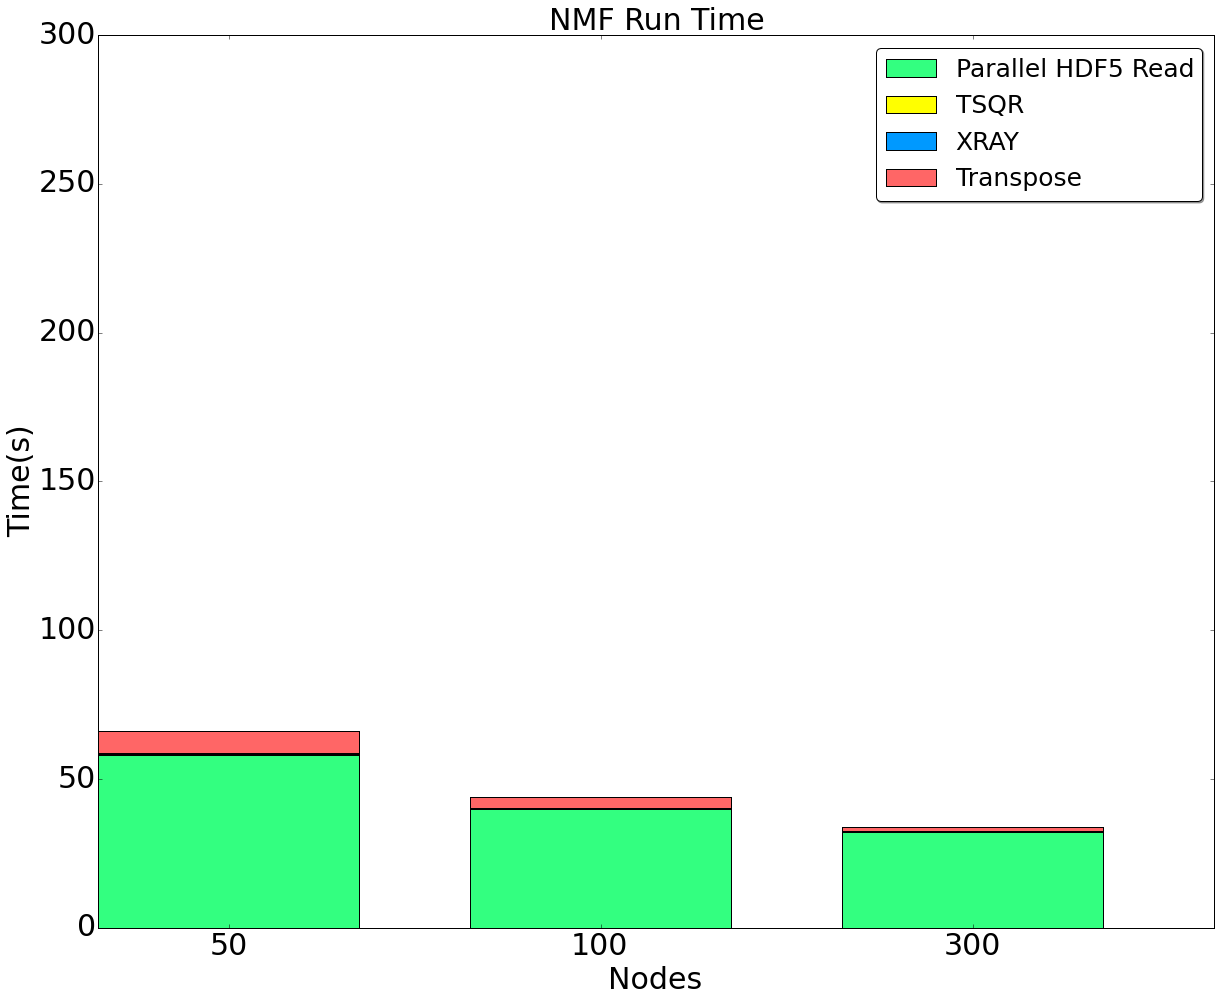
\includegraphics[width=\textwidth]{fig/mpi_nmf_big_scale.png}
\caption{MPI}
\label{fig:mpinmf}
\end{subfigure}
\begin{subfigure}{.4\textwidth}
%\hspace*{\hfill}
%\centering
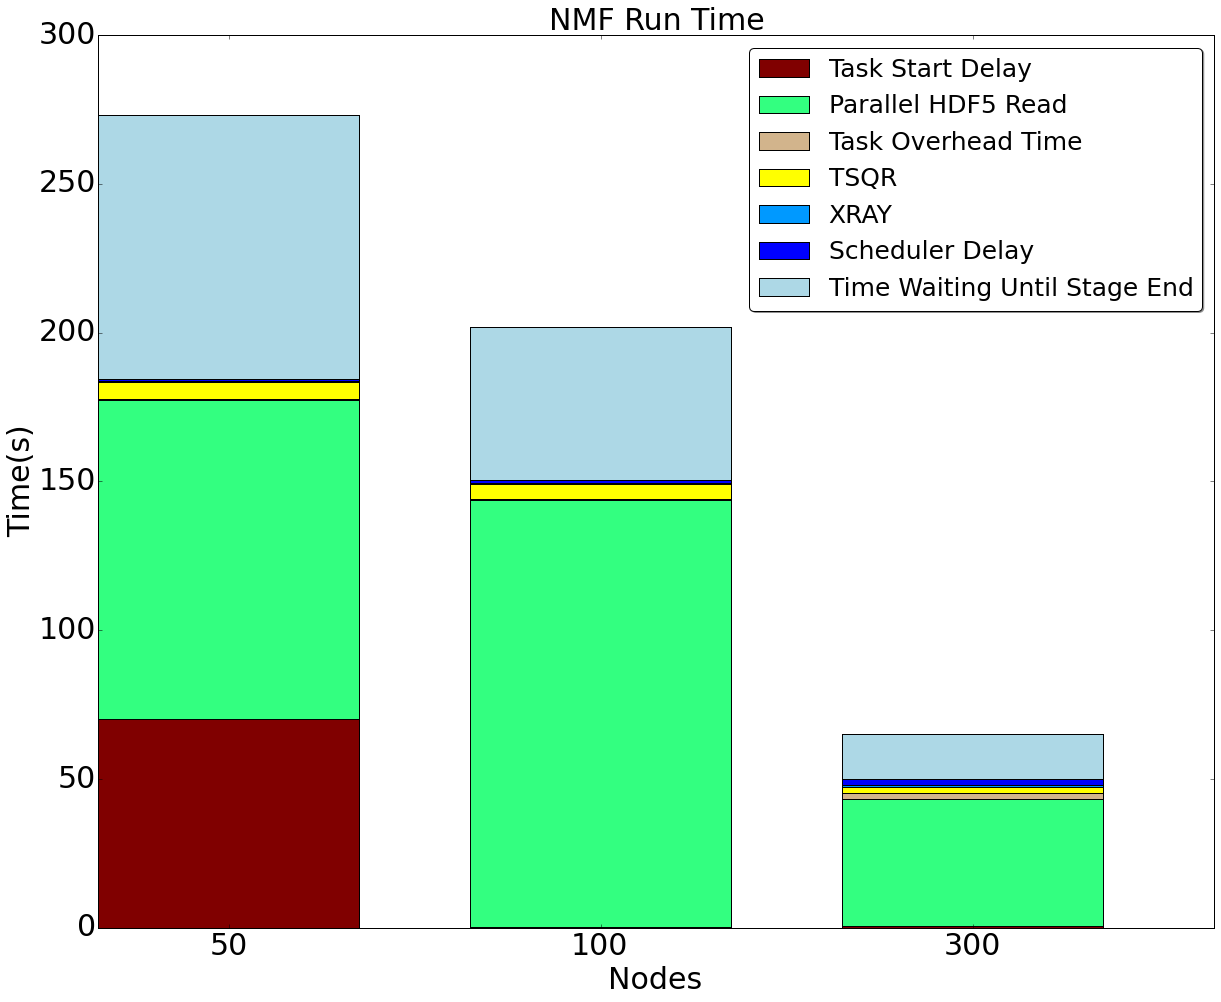
\includegraphics[width=\textwidth]{fig/spark_nmf.png}
\caption{Spark}
\label{fig:nmfspark}
\end{subfigure}
\caption{Running time breakdown of NMF on 1.6TB Daya Bay data at 
node counts of: 50, 100, and 300.}
\label{fig:nmfrt}
\end{figure*}

\begin{figure}[t]
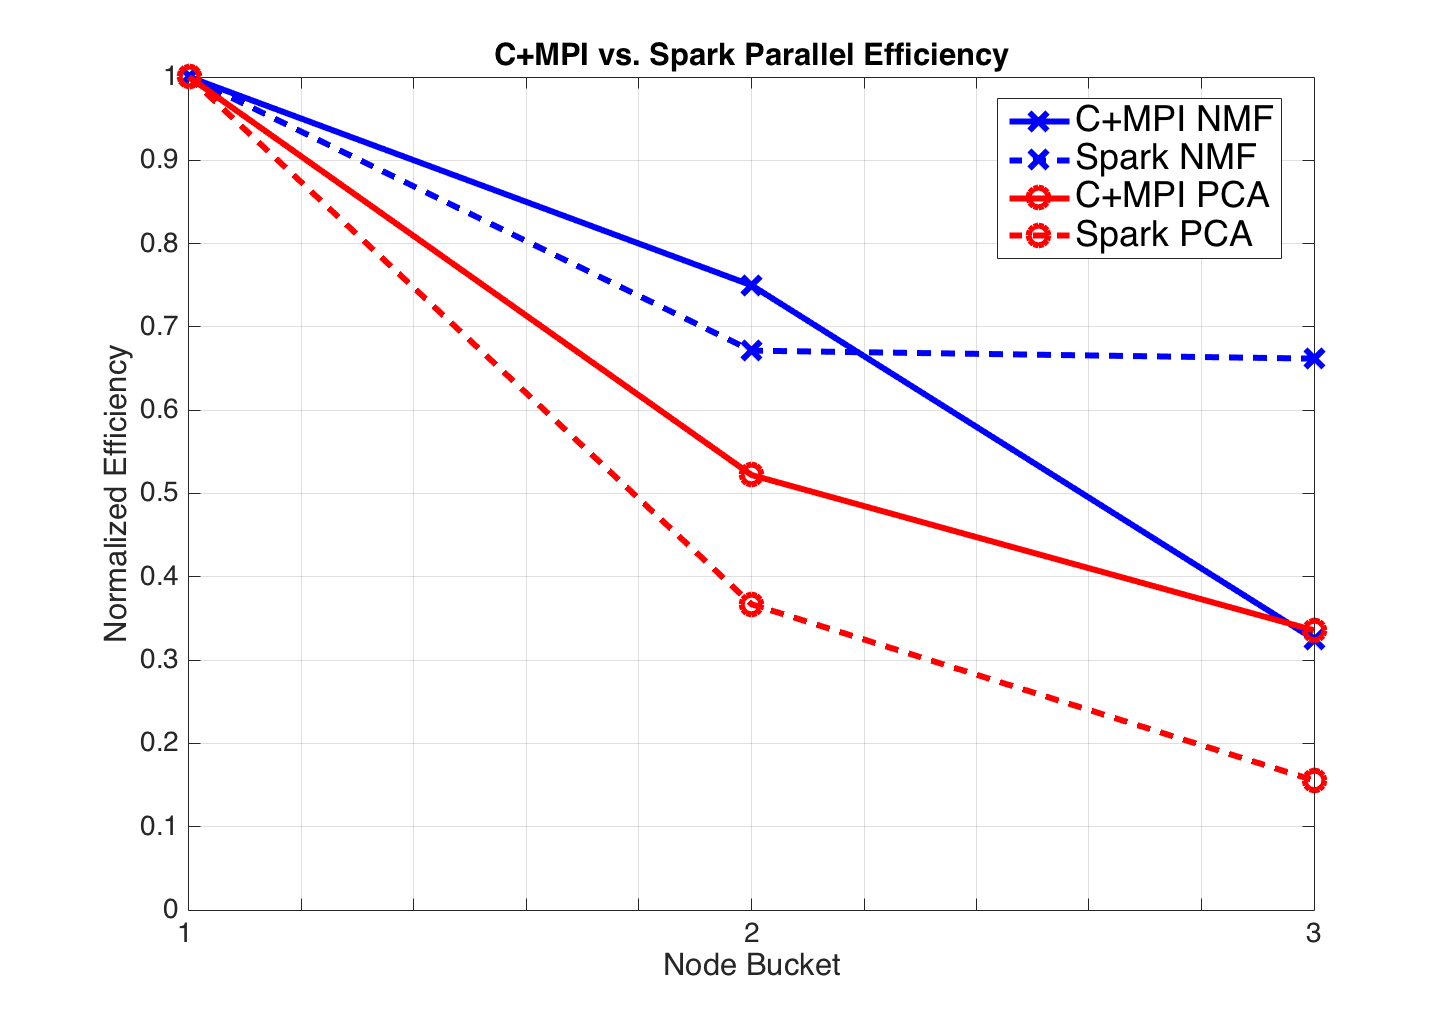
\includegraphics[width=.5\textwidth]{fig/peff.png}
\caption{Comparison of parallel efficiency for C+MPI and Spark. Node count for NMF are 50, 100, and 300 nodes (left to right) and Node count for PCA are 100, 300, and 500 nodes.}
\label{fig:peff}
\end{figure}

\subsection{NMF on Daya Bay}
The separable NMF algorithm we implemented fits nicely into a data parallel programming model. After the initial parallel TSQR the remainder of the algorithm can be computed sequentially. The Daya Bay dataset is especially amenable to this approach due to the extreme aspect ratio of $1B$ rows to $192$ columns.
\subsubsection{C+MPI vs. Spark}
The TSQR algorithm used performs a single round of communication using a flat binary tree with the following, optimal, communication complexity: $O(n^2 \log P)$ words and $O(\log P)$ messages on $P$ processors. Given that the number of columns is very small the NMF algorithm is entirely I/O bound. Figure \ref{fig:mpinmf} shows the running time breakdown of the MPI version of NMF at 50 nodes, 100 nodes, and 300 nodes. The running time for NMF is overwhelmingly dominated by reading the input and, to a lesser degree, the conversion from row-major to column-major layout. TSQR and XRAY have negligible running times in comparison. This combination of dataset and algorithm can be viewed as a test of the I/O subsystems on Cori and the results, a measure of how well those subsystems scale. Figure \ref{fig:mpinmf} shows that the HDF5 read time (in green) does not scale linearly with the number of nodes and is the primary source of inefficiency -- this is due to saturating each OSTs' respective bandwidths. The transpose operation (in red) scales linearly with the number of nodes but represents overhead that can be avoided entirely if the HDF5 interface can perform on-the-fly transposes during reads. XRAY is the sequential bottleneck and costs ~$100$ms at all node counts. TSQR only improves by tens of milliseconds taking $501$ms, $419$ms, and $378$ms at 50, 100, and 300 nodes, respectively. The poor TSQR scaling can be attributed to hitting a communication bottleneck. The TSQR  binary tree is expensive for small matrices especially using flat-MPI. We did not tune our TSQR reduction tree shapes or consider other algorithms since TSQR is not the limiting factor for scalabilty and faster running times. These results illustrate the importance of I/O scalability when performing terabyte-scale data parallel analytics on a high-performance architecture using MPI.

Figure \ref{fig:nmfspark} illustrates the running time breakdown for Spark NMF on 50, 100, and 300 nodes. Unlike C and MPI, Spark incurs significant overhead for task scheduling, task start delays and idle time due to Spark stragglers. For the 50 node run we configured Spark to use double the number of partitions as physical cores because we encountered out-of-memory errors for fewer partitions. The number of partitions was not doubled for the 100 and 300 node runs. Similar to the C and MPI results, most of the running time is dominated by I/O and Spark overheads with a small amount of time spent in TSQR and XRAY. The Spark version does not include an explicit transpose because it is handled by the Breeze library when making a call to optimized BLAS during TSQR. Figure \ref{fig:nmfspark} shows that Spark NMF exhibits good strong scaling behavior up to 300 nodes.  Even though NMF is entirely data parallel and suitable for Spark, we observed a $4\times$, $4.6\times$, and $2.3\times$ performance gap on 50, 100, and 300 nodes, respectively, between Spark and MPI.

Figure \ref{fig:peff} shows the parallel efficiency of MPI NMF and Spark NMF. The parallel efficiency results are normalized to the 50 node running time of the respective parallel frameworks to measure their scaling efficiency. MPI NMF is completely dominated by I/O and the results are primarily indicative of scaling issues in the I/O subsystem. Spark NMF displays good scaling with more nodes and this is reflected in the parallel efficiency. However, the scaling is due to decreases -- in some cases drastic decreases --  in Spark overhead, delays and straggler effects. If Spark NMF running times are normalized against MPI NMF then the parallel efficiency drops sharply to below 20\% for all node counts. This indicates that Spark does not push the available hardware to its limits and spends much of its running time on overheads.

%\begin{figure}[t]
%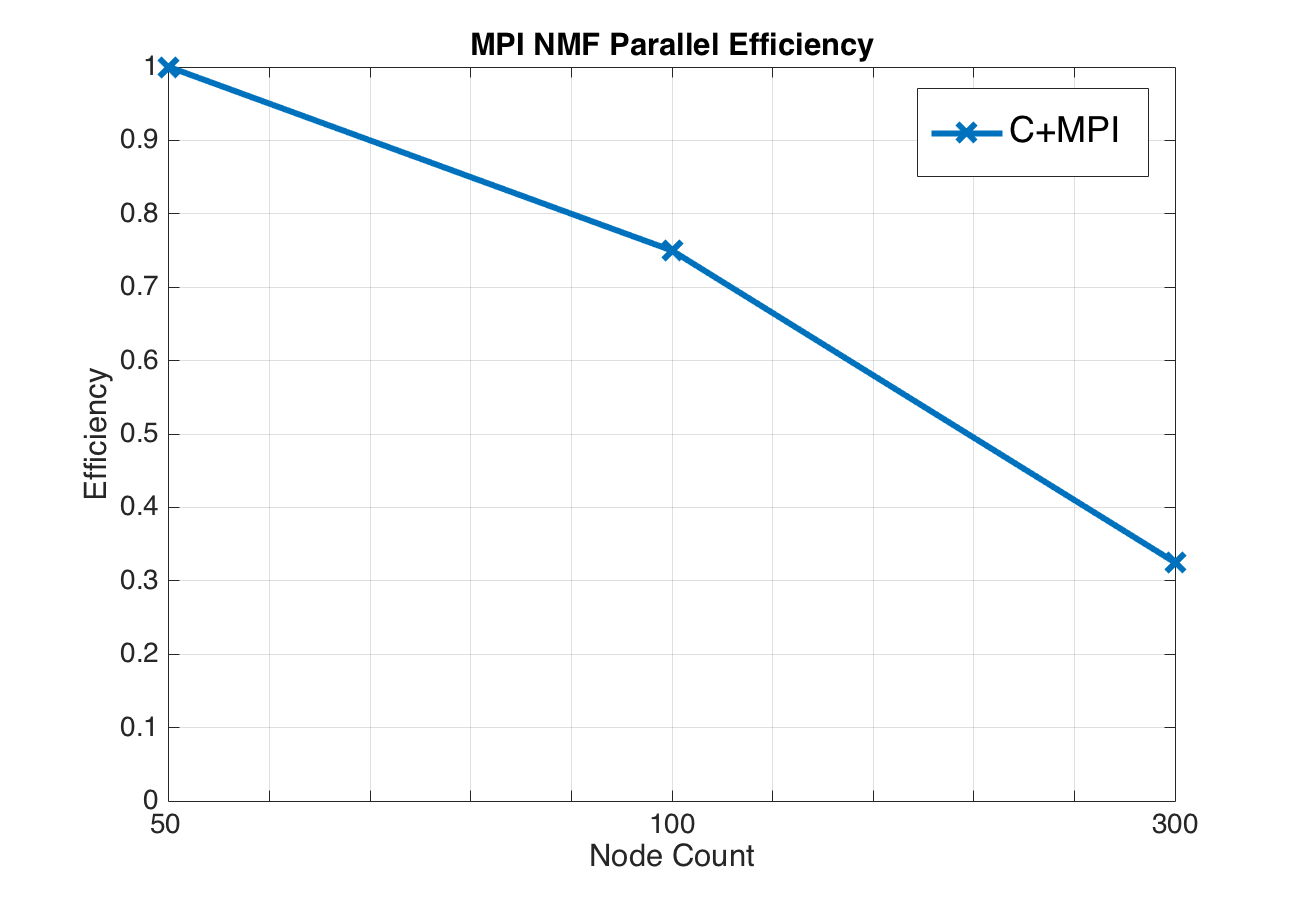
\includegraphics[width=.5\textwidth]{fig/nmf_peff.png}
%\caption{Comparison of parallel efficiency for Spark NMF and MPI NMF.}
%\label{fig:nmfpeff}
%\end{figure}

%\textcolor{blue}{parallel efficiency, stacked bar graph of running time.}

%   \begin{figure}[t]
%   \includegraphics[width=.5\textwidth]{fig/nmf_timeline.png}
%   \end{figure}


\subsubsection{Science Interpretation}
We are currently investigating the results of the NMF decomposition. Preliminary analysis of the results indicates that we might need to augment the input datasets with non-linear feature descriptors (Kernel methods) to make the input signals invariant to rotations and translations. Our eventual goal is to learn event-specific classifiers from the coefficients of the basis vectors. The classification will enable us to accomplish the final goal of segmenting and labeling the timeseries. While successfully implementing the entire pipeline is somewhat out of scope for this submission, the fact that we have determined basis vectors from the TB-sized dataset will enable us to explore more advanced methods in the near future.

\subsection{PCA on Climate}
\begin{figure*}[th!]
\begin{subfigure}{.45\textwidth}
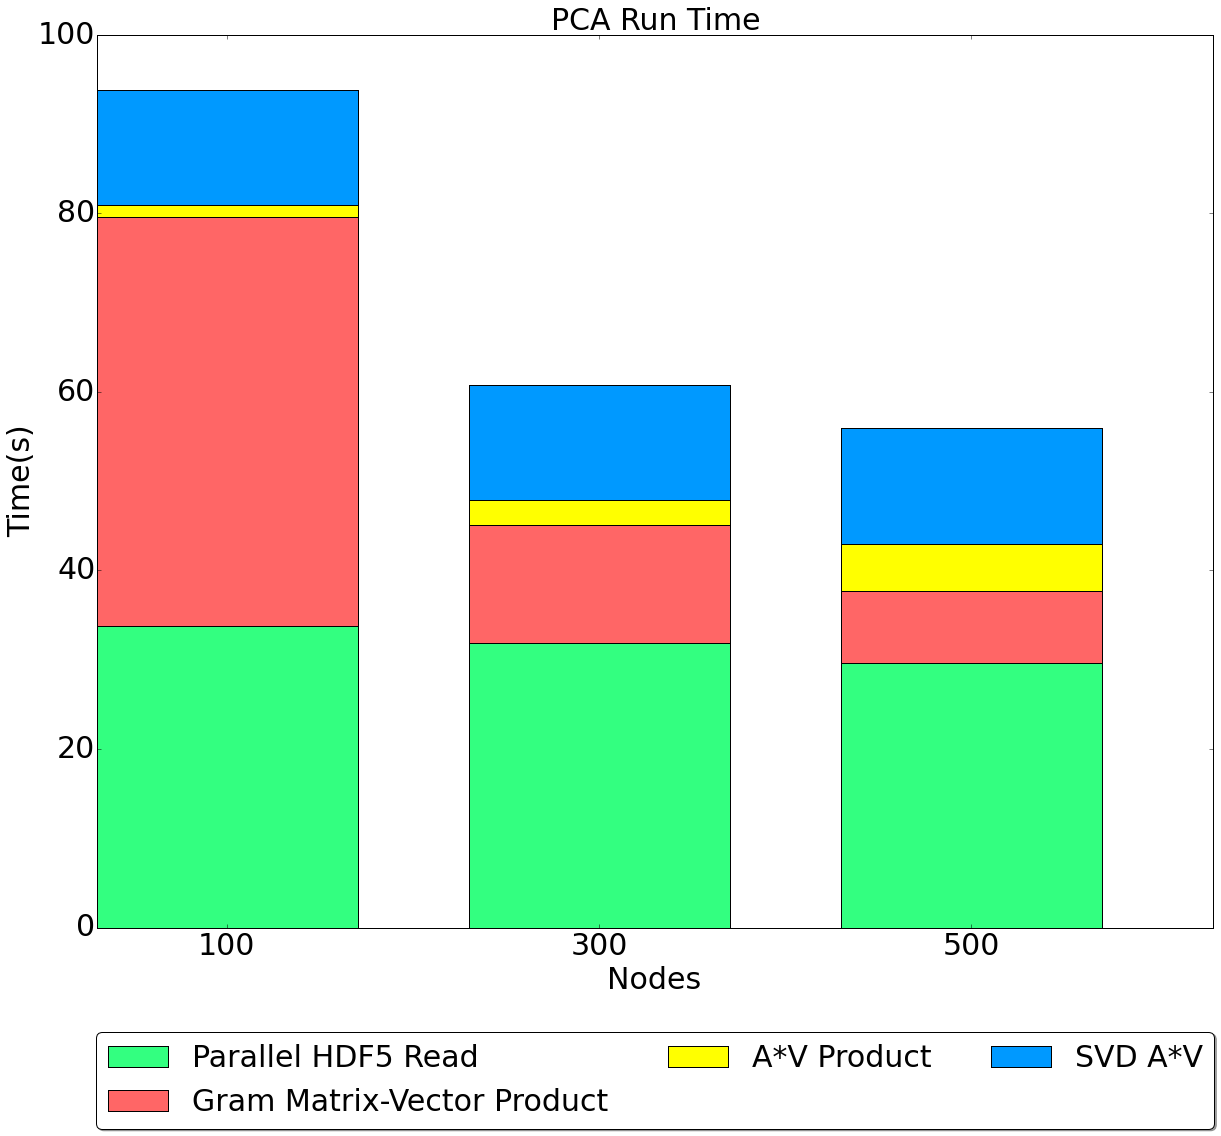
\includegraphics[width=\textwidth]{fig/mpi_pca.png}
\caption{MPI}
\label{fig:mpipca}
\end{subfigure}
\begin{subfigure}{.5\textwidth}
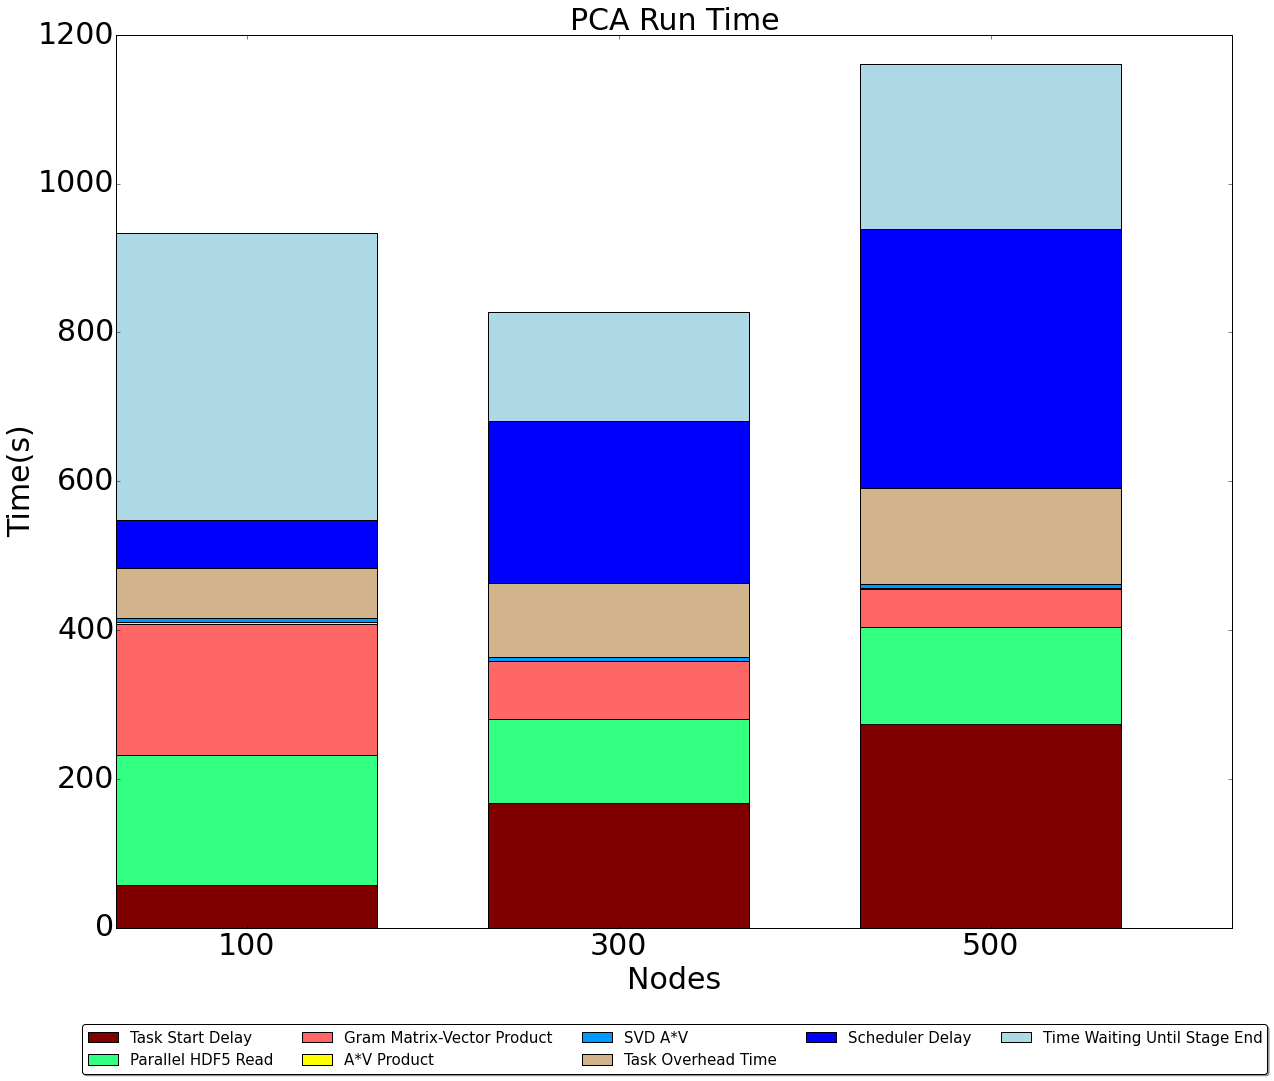
\includegraphics[width=\textwidth]{fig/spark_pca.png}
\caption{Spark}
\label{fig:sparkpca}
\end{subfigure}
\caption{Running time breakdown of PCA on 2.2TB Ocean data at node counts of: 100, 300 and 500.}
\label{fig:pcart}
\end{figure*}

PCA is an iterative algorithm which requires an SVD of the data matrix in order to find its top-$k$ left singular vectors. The main kernel of this algorithm is a distributed matrix-vector product at every iteration. Since matrix-vector products are data parallel, the PCA algorithm also fits into the Spark model. The additional requirement for PCA is that the data matrix needs to be cached in memory on Spark to avoid I/O at each iteration.

\subsubsection{C+MPI vs. Spark}
%The C and MPI version reads the dataset from a single HDF5 file, computes a rank-$k$ eigenvalue decomposition, EVD, ($V\Lambda V^T$) of the Gramian matrix $A^TA$ in parallel, performs a parallel matrix-matrix multiplication ($AV$) and, finally, a sequential singular value decomposition of $AV$. Once again, the matrix is partitioned into a 1D-block row decomposition. We use arpack-ng \cite{Lehoucq97} to compute the EVD which requires a user-defined function to perform matrix-vector products. We do this by first broadcasting the Lanczos vector $x$ to all processors and compute a local matrix-vector product. This results in a vector $y = Ax$ distributed across different processors, from which the vector $z = A^Ty$ can be computed. $z$ is formed by computing partial matrix-vector products using locally stored blocks of $A$ and $y$, which are then globally summed using an \verb+MPI_Allreduce+. This process is repeated until the Lanczos method converges -- we set the tolerance to $10^{-13}$. After convergence the $k$ eigenvectors just computed are broadcasted to all processors which compute partial matrix-matrix products that are globally summed. Finally,  we compute a sequential SVD to obtain the top-$k$ left singular vectors of $A$. 
Figure \ref{fig:mpipca} shows the running time breakdown results for PCA on 100, 300, and 500 nodes. I/O is a significant bottleneck and does not exhibit the scaling observed for NMF in Figure \ref{fig:mpinmf}. However, the absolute I/O time for NMF and PCA are consistent which suggests that the I/O bandwidth is saturated for the stripe size used for the Daya Bay and Ocean datasets. The Gram matrix-vector products are a significant portion of the running time but scale linearly with the number of nodes. The matrix-matrix product ($AV$) does not scale due to a communication bottleneck. The bottleneck is because we compute a rank-$20$ PCA which makes communicating $V$ very expensive. This cost grows with the number processors since it is entirely latency dominated. The final SVD of $AV$ is a sequential bottleneck and does not scale. Unlike NMF the sequential bottleneck in PCA is significant and future implementations should perform this step in parallel.

Figure \ref{fig:sparkpca} shows the scaling and running time breakdown of the Spark PCA implementation for 100, 300, and 500 nodes. The Gram matrix-vector products scale linearly with the number of nodes however this is outweighed by inefficiencies in Spark. At this scale, Spark is entirely bottlenecked by scheduler delays, task overhead and Spark straggler delay times. Task overhead consists of deserializing a task, serializing a result and writing and reading shuffle data. The Spark scheduling delay and task overhead time scales inversely with the number of nodes. This is likely due to the centralized scheduler used in Spark. PCA is a data parallel algorithm, however, its iterative nature stresses the Spark scheduler since many tasks are launched during each iteration. Under this workload we observed a 10.2$\times$, 14.5$\times$, and 22$\times$ performance gap on 100, 300, and 500 nodes, respectively, between Spark and MPI.

Figure \ref{fig:peff} shows the parallel efficiency of MPI PCA and Spark PCA. In the PCA case we observed that the MPI version hits an I/O bottleneck, a communication bottleneck in the $AV$ product and a sequential bottleneck in SVD($AV$). All of these are limiting factors and introduce inefficiencies to MPI PCA. The Spark PCA running time are normalized to the running time of Spark PCA at 100 nodes. As before, this normalization illustrates how efficient Spark is with more nodes. Spark PCA is less efficient that MPI PCA due to scheduler delays, task overhead and straggler effects. The scheduler delays are more prominent in PCA than in NMF due to the larger number of tasks. NMF makes a single pass over the data whereas PCA makes many passes over the data and launches many tasks per iteration.
% \begin{figure}[t]
% 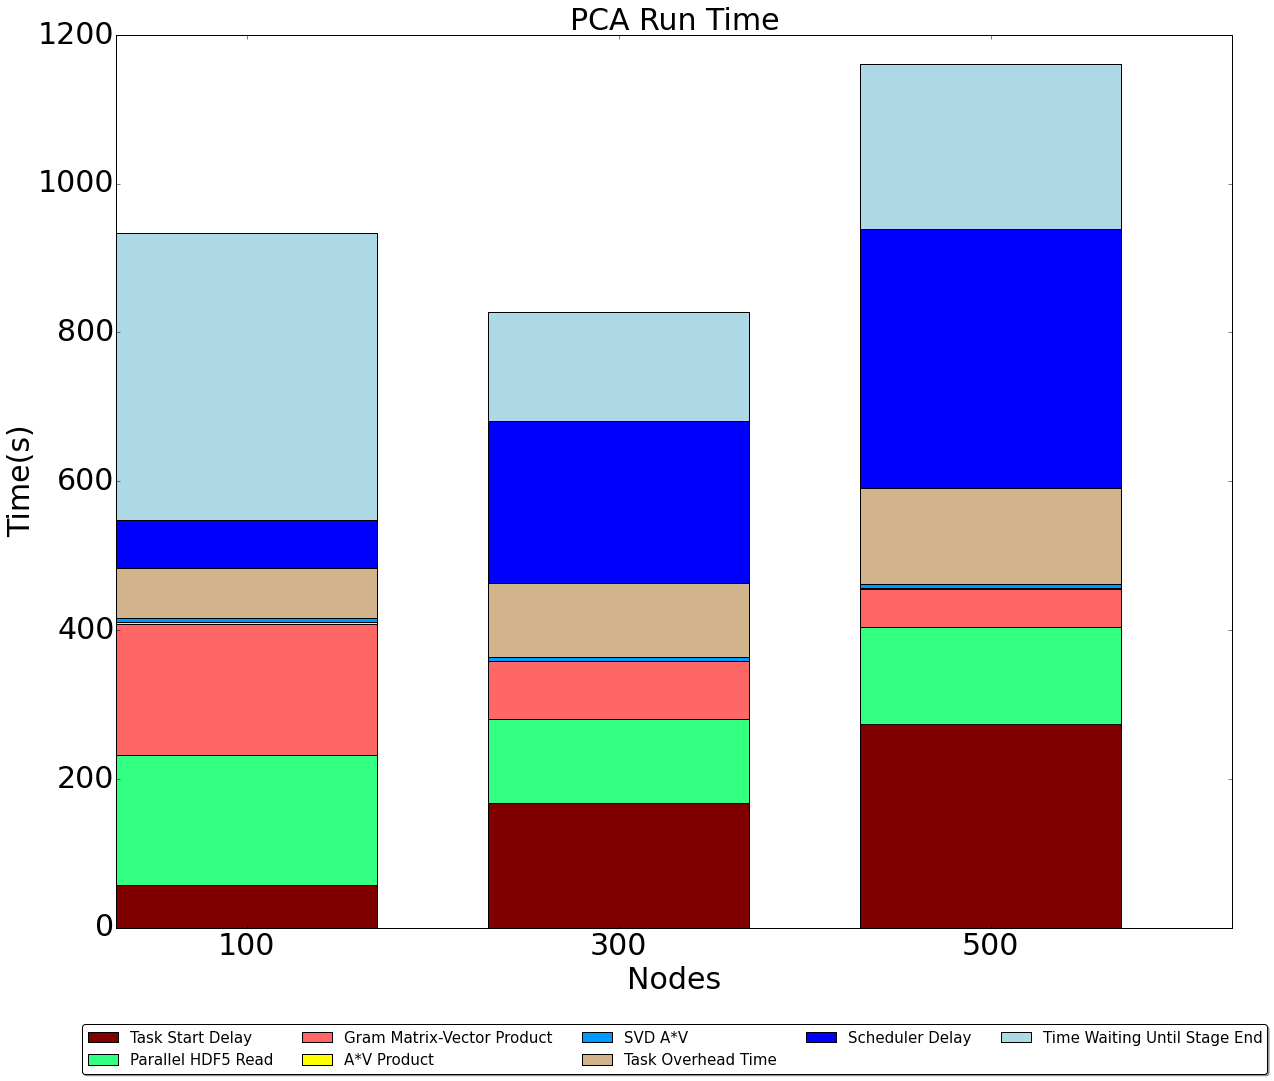
\includegraphics[width=.5\textwidth]{fig/spark_pca.png}
% \end{figure}


% \begin{figure}[t]
% 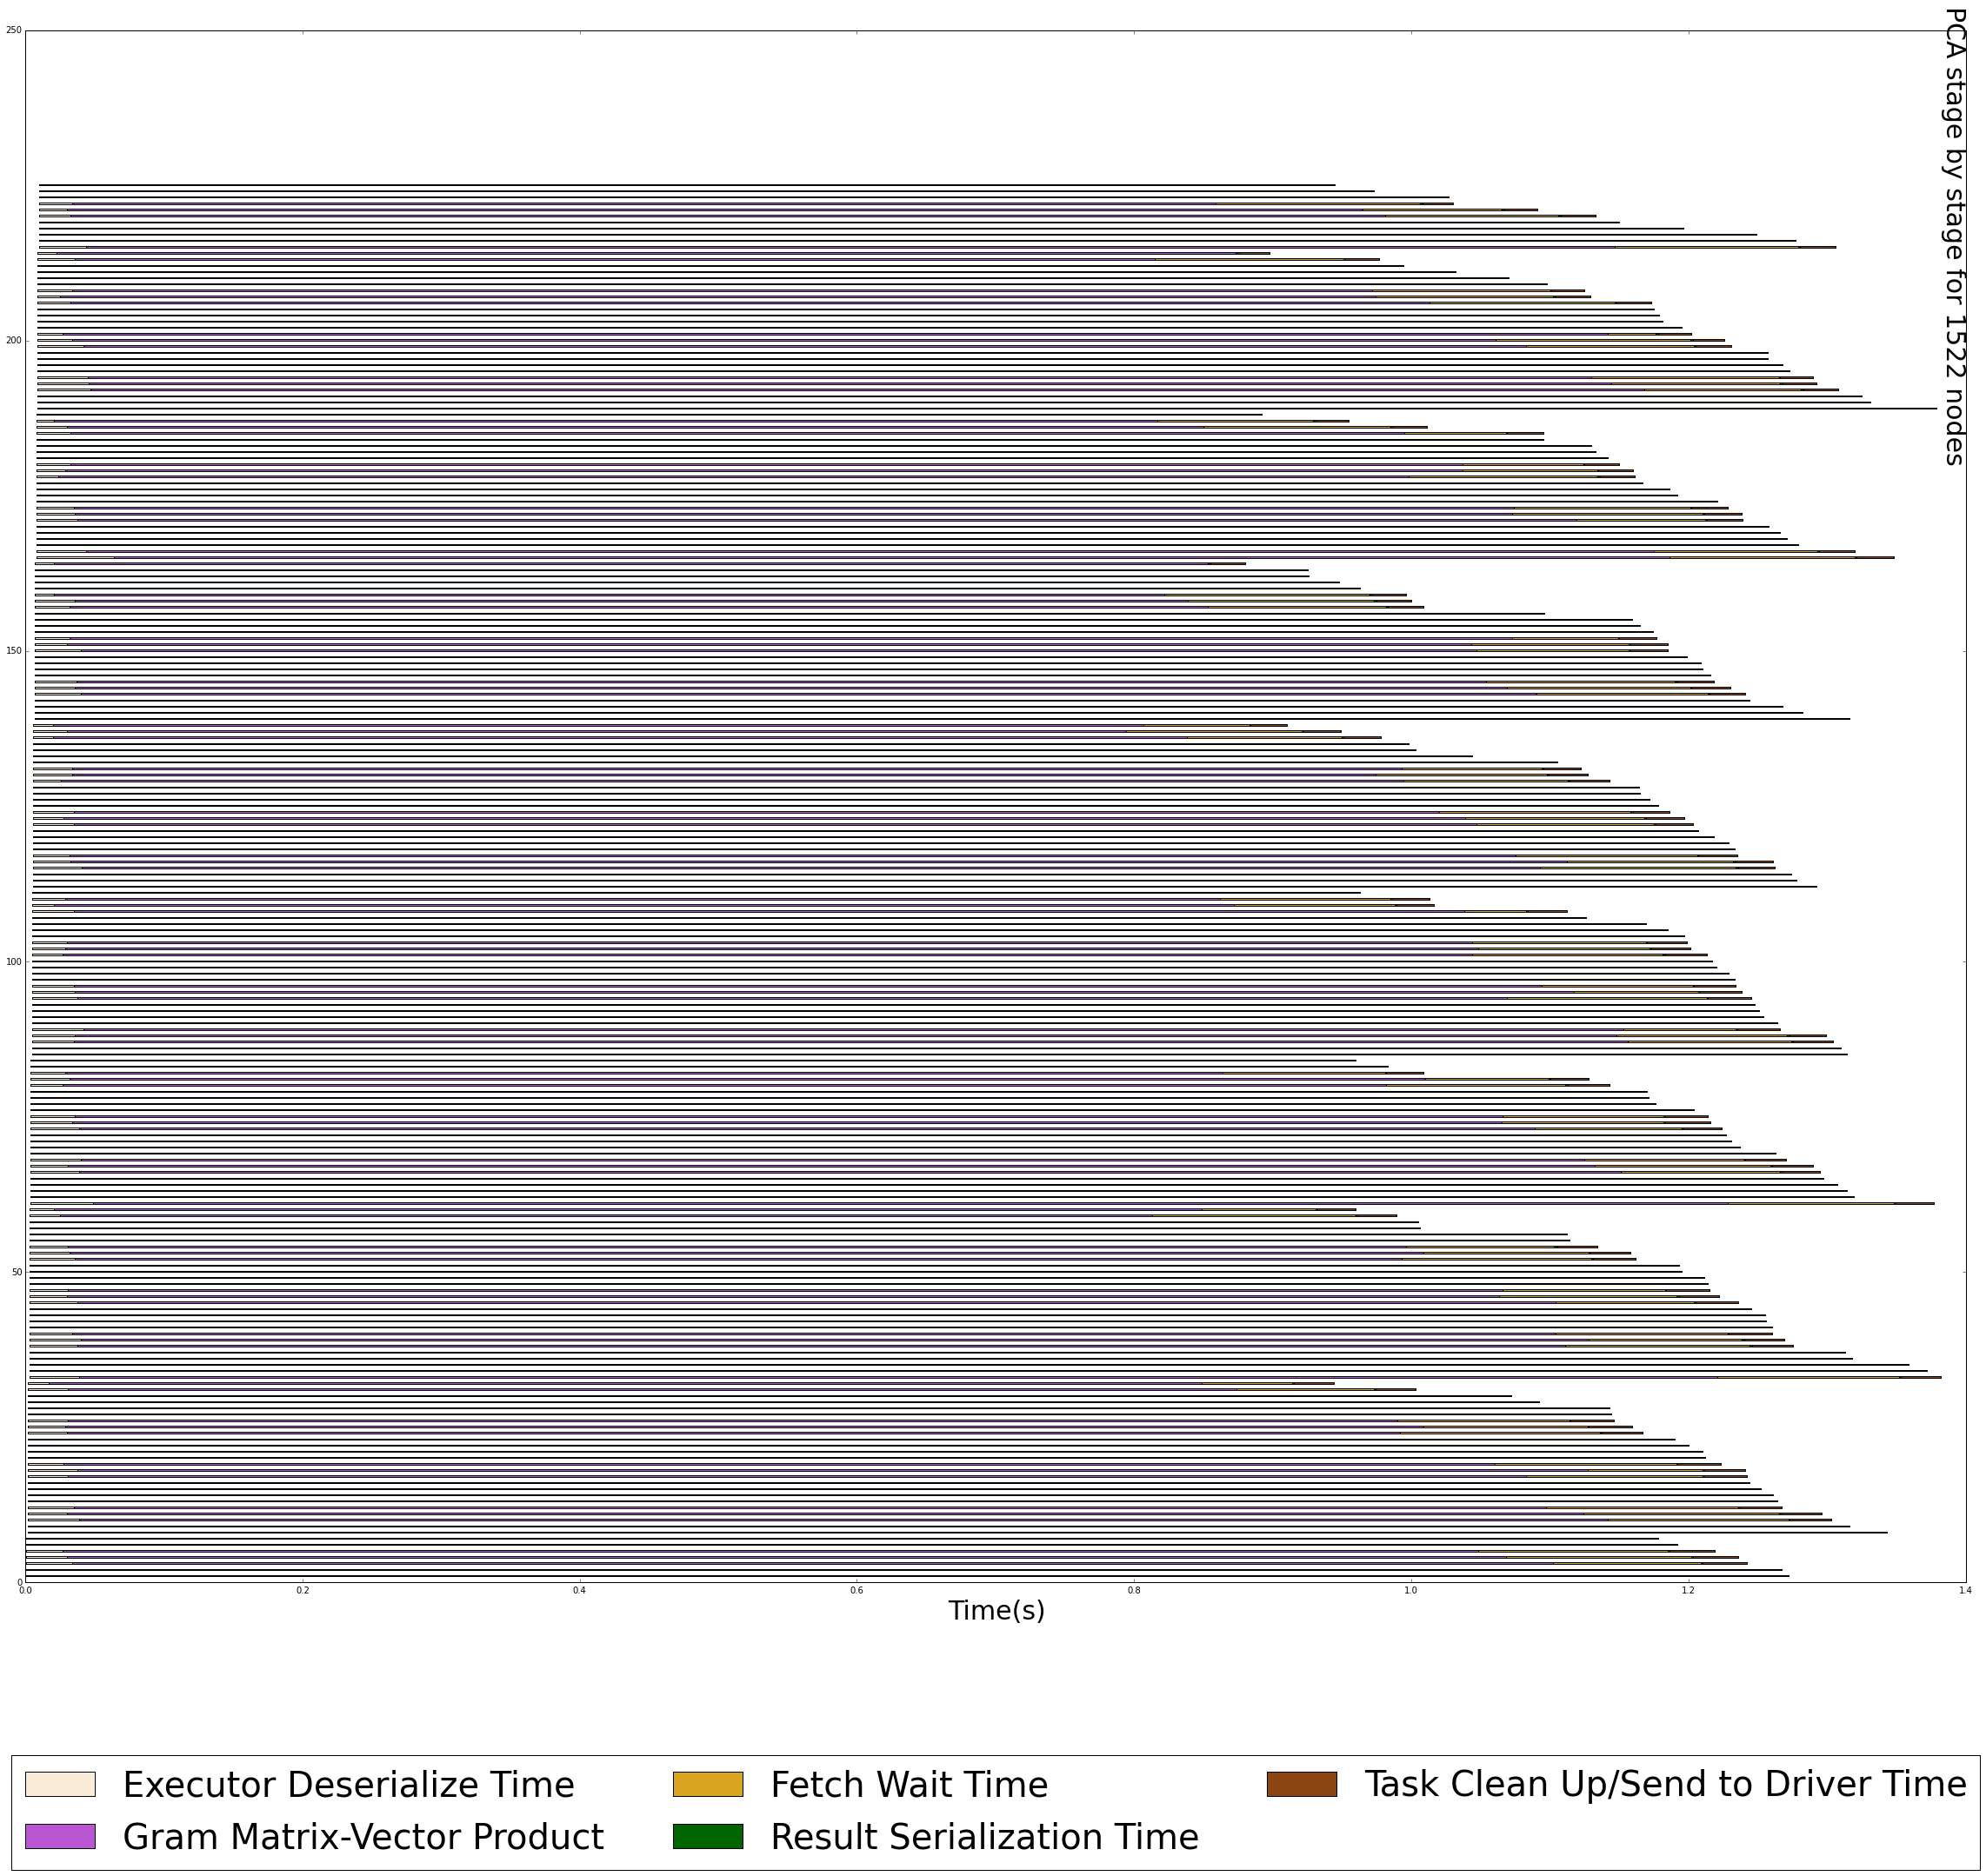
\includegraphics[width=.5\textwidth]{fig/stage_8_hero_run.png}
% \end{figure}

%\textcolor{blue}{parallel efficiency, stacked bar graph of running time.}
\subsubsection{Hero Run}
\begin{figure}[th]
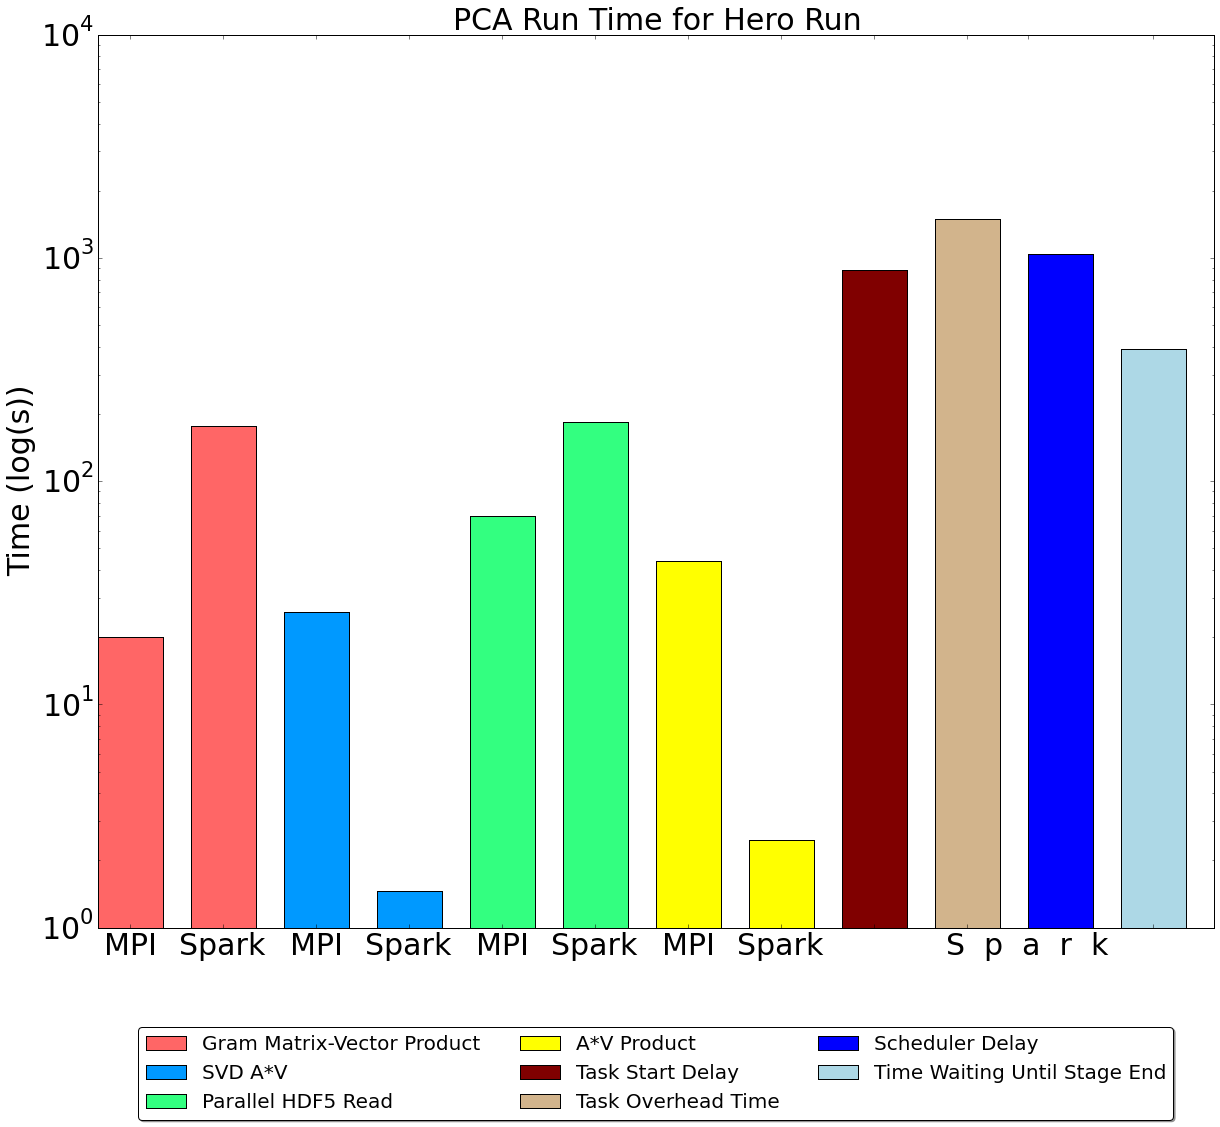
\includegraphics[width=.5\textwidth]{fig/hero_run_summary.png}
\caption{Running time comparison of MPI PCA and Spark PCA for Hero run.}
\label{fig:hero}
\end{figure}
For this run we use all 1600 nodes for Cori to perform PCA on 16TB of Atmosphere data. In order to complete this benchmark in a reasonable amount of time, we fix  the number of iterations for the EVD of $A^TA$ to $70$ iterations. MPI PCA was able to complete this run in $160s$. Unfortunately we were unsuccessful at launch Spark on $1600$ nodes and after many attempts we reduced the number of nodes to $1522$. Once the node count was decreased Spark PCA successfully completed the run in $4175s$. Figure \ref{fig:hero} shows the head-to-head running time comparison of the full-system run.   

\subsubsection{Science Interpretation}
The first two temporal EOFs, corresponding to $V_k$, fully capture the annual cycles. The remaining time series show abrupt changes due to the 1983 ENSO, and more significantly, the record-breaking ENSO of 1997--98. The intermediate modes contain a complex interplay of various timescales, which is currently under investigation. The spatial EOFs, corresponding to $U_k$, show the relative dominance of the Indian Ocean Dipole and the classic warm pool--cold tongue patterns of ENSO at various depths below the ocean surface. Because of the 3D nature of the EOFs, we are able to see that the dynamic near the thermocline is most dominant, rather than that closer to the surface. Further, there are several smaller scale features that have a strong influence at different depths. Work is on-going to understand the nature of these different spatial patterns and the factors that influence their relative dominance.

\subsection{CX on Mass-spec Imaging}
\begin{table}[t]
\begin{center}
\resizebox{\columnwidth}{!}{
\begin{tabular}{|c|c|c|c|} \hline
Algo & Size & \# Nodes & Spark Time (s)\\ \hline
\multirow{3}{*}{CX} & \multirow{3}{*}{1.1 TB} & $60$ & $1200$\\
{} & {} & $100$  & $784$\\
{} & {} & $300$ & $542$\\ \hline
% {} & \multirow{3}{*}{Spark} & {} & $221$ & $122$ & $032$\\
% {} & {} & \multirow{2}{*}{$311$} & $212$ & $131$ & $023$\\
% {} & {} & {} & {} & $113$ & $050$\\
\end{tabular}
}
\end{center}
\caption{Spark CX running times}
\label{tab:cxscale}
\end{table}
Much like PCA, the CX decomposition requires a parallel Gramian multiply, a distributed matrix-matrix product and a randomized SVD in order to compute extremal columns of $A$. CX is applied to the 1.1TB MSI dataset stored as a file in native Spark Parquet format. Table \ref{tab:cxscale} shows the running times and scaling behavior of Spark CX. We found that Spark exhibited good scaling for the range of nodes tested and attained speedups of $1.5\times$ and $2.2\times$ on 100 and 300 nodes, respectively. 
\subsubsection{Science Interpretation}
 The CX decomposition selected ions in three narrow regions of $m/z$. Among those ions identified as having significant leverage scores are ions at $m/z$ values of 439.0819, 423.0832, and 471.1276, which correspond to neutral losses of $\rm{CH_2}$, $\rm{CH_2O}$, and a neutral ``gain'' of $\rm{H_2O}$ from the 453.0983 ion.  These relationships indicate that this set of ions, all identified by CX as having significant leverage scores, are chemically related.  That fact indicates that these ions may share a common biological origin, despite having distinct spatial distributions in the plant tissue sample.  

 \subsection{Summary of Spark vs. C+MPI performance comparison}
 \begin{table}[t]
\begin{center}
\resizebox{\columnwidth}{!}{
\begin{tabular}{|c|c|c|c|} \hline
Algo & \# Nodes & Gap with I/O & Gap without I/O\\ \hline
\multirow{3}{*}{NMF} & $50$ & $4\times$ & $21.2 \times$\\
{} & $100$  & $4.6\times$ & $14.9\times$\\
{} & $300$ & $2.3\times$ & $15.7\times$\\ \hline
\multirow{4}{*}{PCA} & 100 & $10.2\times$ & $12.6\times$\\
 {} & 300 & $14.5\times$ & $24.7\times$\\
 {} & 500 & $22\times$ & $39.3\times$\\ \cline{2-4}
 {} & {MPI: 1600 Spark: 1522} & $26\times$ & $43.8\times$\\ \hline
% {} & \multirow{3}{*}{Spark} & {} & $221$ & $122$ & $032$\\
% {} & {} & \multirow{2}{*}{$311$} & $212$ & $131$ & $023$\\
% {} & {} & {} & {} & $113$ & $050$\\
\end{tabular}
}
\end{center}
\caption{Overall summary of MPI and Spark performance gaps.}
\label{tab:perfgaps}
\end{table}
We've shown in this section that matrix factorizations which have traditionally been implemented using high-performance parallel framework can be implemented on Spark and that Spark can run on large node counts on high-performance platforms. By exploring the performance tradeoffs of Spark matrix factorizations and comparing to traditional MPI implementations we have gained key insights into Spark's scalability. Table \ref{tab:perfgaps} summarizes the performance gaps between Spark and MPI which are $2-25\times$ with I/O times and $10-40\times$ without I/O times. Though the gaps may be large, our experiments indicated that Spark I/O scaling is comparable to MPI I/O scaling, that the computation phases exhibit good strong scaling and that many of the bottlenecks are a result of scheduler delays, straggler effects and task overhead times. If these bottlenecks can be alleviated, then Spark can close the performance gap and become a competitive, easy-to-use framework for data analytics on high-performance architectures.   

 %\textcolor{red}{Mike, Kristi, Aditya}
 %\begin{itemize}
 %\item{Call out 7-25x performance gap}
 %\item{Call out comparable I/O performance}
 %\item{Call out scaling of compute steps in Spark}
 %\item{Call out overhead issues in Spark}
 %\item{Call out other system issues?}
%\end{itemize}

%\textcolor{blue}{We'll only want to comment on comparative performance issues here and leave all Spark-specific discussions to Section VII.}
        

\section{Lessons Learned}
\label{sec:lessons}
Throughout the course of these experiments, we have learned a number of lessons pertaining to the behavior of Spark for linear algebra computations in large scale HPC systems. 
In this section, we share some of these lessons and conjecture on likely causes.
\paragraph{Spark Scheduling Bottlenecks.}
%There are two main sources of sequential bottleneck in Spark: Task Start Delay and Scheduler Delay. Task Start delay for a particular task is the time from the start of the stage to when the scheduler creates and sends out the task to an executor. Because tasks are created one by one by the driver as it checks resources to see where to send them, higher concurrency leads to high task start delays. Scheduler delay consists of two items: the time it takes for the executor to receive the message to start as task and spawn a thread and the time it takes for the task to send a message back to the driver. Scheduler delay is known to be either caused by large tasks or large results, which slow down the sending process. In our case, however, we believe that a big part of the scheduler delay we observe increasing as we increase concurrency is due to the large number of tasks we are launching at once. This causes delay as many task completed messages are sent back to the driver at once and are queued as they are processed one by one. 
The Spark driver creates and sends tasks serially, which can cause bottlenecks at high concurrency.  This can be measured by looking at two metrics: Task Start Delay and Scheduler Delay. Task Start Delay measures the time until the  task is sent to an executor. Scheduler Delay measures the additional time until the driver receives confirmation that the task has been received and begun execution. Figure~\ref{fig:hero-timeline} is a plot of a sample of tasks from one stage of the PCA hero run.  Note that the ordering of the colored bars within each task line does not correspond to the order they occurred---Spark uses a pipelined execution model, where different portions of a task are interleaved at a fine grain, and then reports back total times spent on each activity.  We can see that this scheduling bottleneck causes a uniform distribution of start times, with tasks starting as late as 20 seconds after the earliest task.  The scheduler delay appears inversely proportional to start delay, indicating that confirmation messages are queuing up and waiting to be processed at the driver while it finishes sending new tasks.

\begin{table}[th]
\centering
\begin{tabular}{| c | c | c | c | c | c | c |}
\hline
Algo & Size & Nodes & Partitions & Time (s) & Measured & Predicted \\
{} & {} & {} & {} & {} & Task Start & Delay \\
{} & {} & {} & {} & {} & Delay (s) & (2000/sec) \\
\hline
\multirow{4}{*}{PCA} & \multirow{3}{*}{2.2 TB} & 100 & 3200 & 924 & 411 & 112 \\
 {} & {} & 300 & 9600 & 827 & 332 & 336 \\
 {} & {} & 500 & 16000 & 1160 & 542 & 560 \\ \cline{2-7} & & & & & & \\[-1ex]
 {} & {16 TB} & 1522 & 51200 & 3718 & 1779 & 1792 \\
 \hline
\end{tabular}
\caption{Spark scheduling delays.}
\label{tab:scheduling}
\end{table}

Ousterhout et al.~\cite{Ousterhout13Sparrow} showed that these factors limit the Spark scheduler to launching approximately 1500 tasks per second.  Their measurements were based on an older version of Spark from 2013.  There have not been significant changes to the scheduler, however, and our results on Cori are consistent with a similar rate of about 2000 tasks per second.  We show the impact of this bottleneck on PCA in Table~\ref{tab:scheduling}.  
We expect the largest impact on scaling here, due to the need to schedule 70 iterations.  Each iteration contains an initial stage that must schedule a task for every partition.  The \emph{Measured Task Start Delay} column shows the sum of the largest task start delays in each Spark stage.  The \emph{Predicted Delay} column shows the delay predicted by a scheduling rate of 2000 tasks per second over 70 iterations and the listed number of tasks/partitions.  We observe that at 300, 500, and 1522 nodes, the task start delay is very close to the predicted~value.%\footnote{At 100 nodes, we see a delay that is much higher than predicted, indicating that an additional source of delay has contributed.  In particular, there was a single task with a delay of 90 seconds during that run, which alone accounts for almost a third of the difference from the predicted value.}

This bottleneck represents a limit on the scaling achievable by Spark for highly iterative algorithms.  In particular, as the amount of parallelism increases, the minimum number of partitions and tasks also increases.  This results in a linearly increasing overhead from the scheduler as we increase parallelism.  This delay is further multiplied by the number of stages.  We see the impact of this in the PCA results in Table~\ref{tab:scheduling}, where the final column represents this fixed overhead and is thus a lower bound on how fast we can execute at the given scale.  


\begin{figure}[tbhp]
\centering
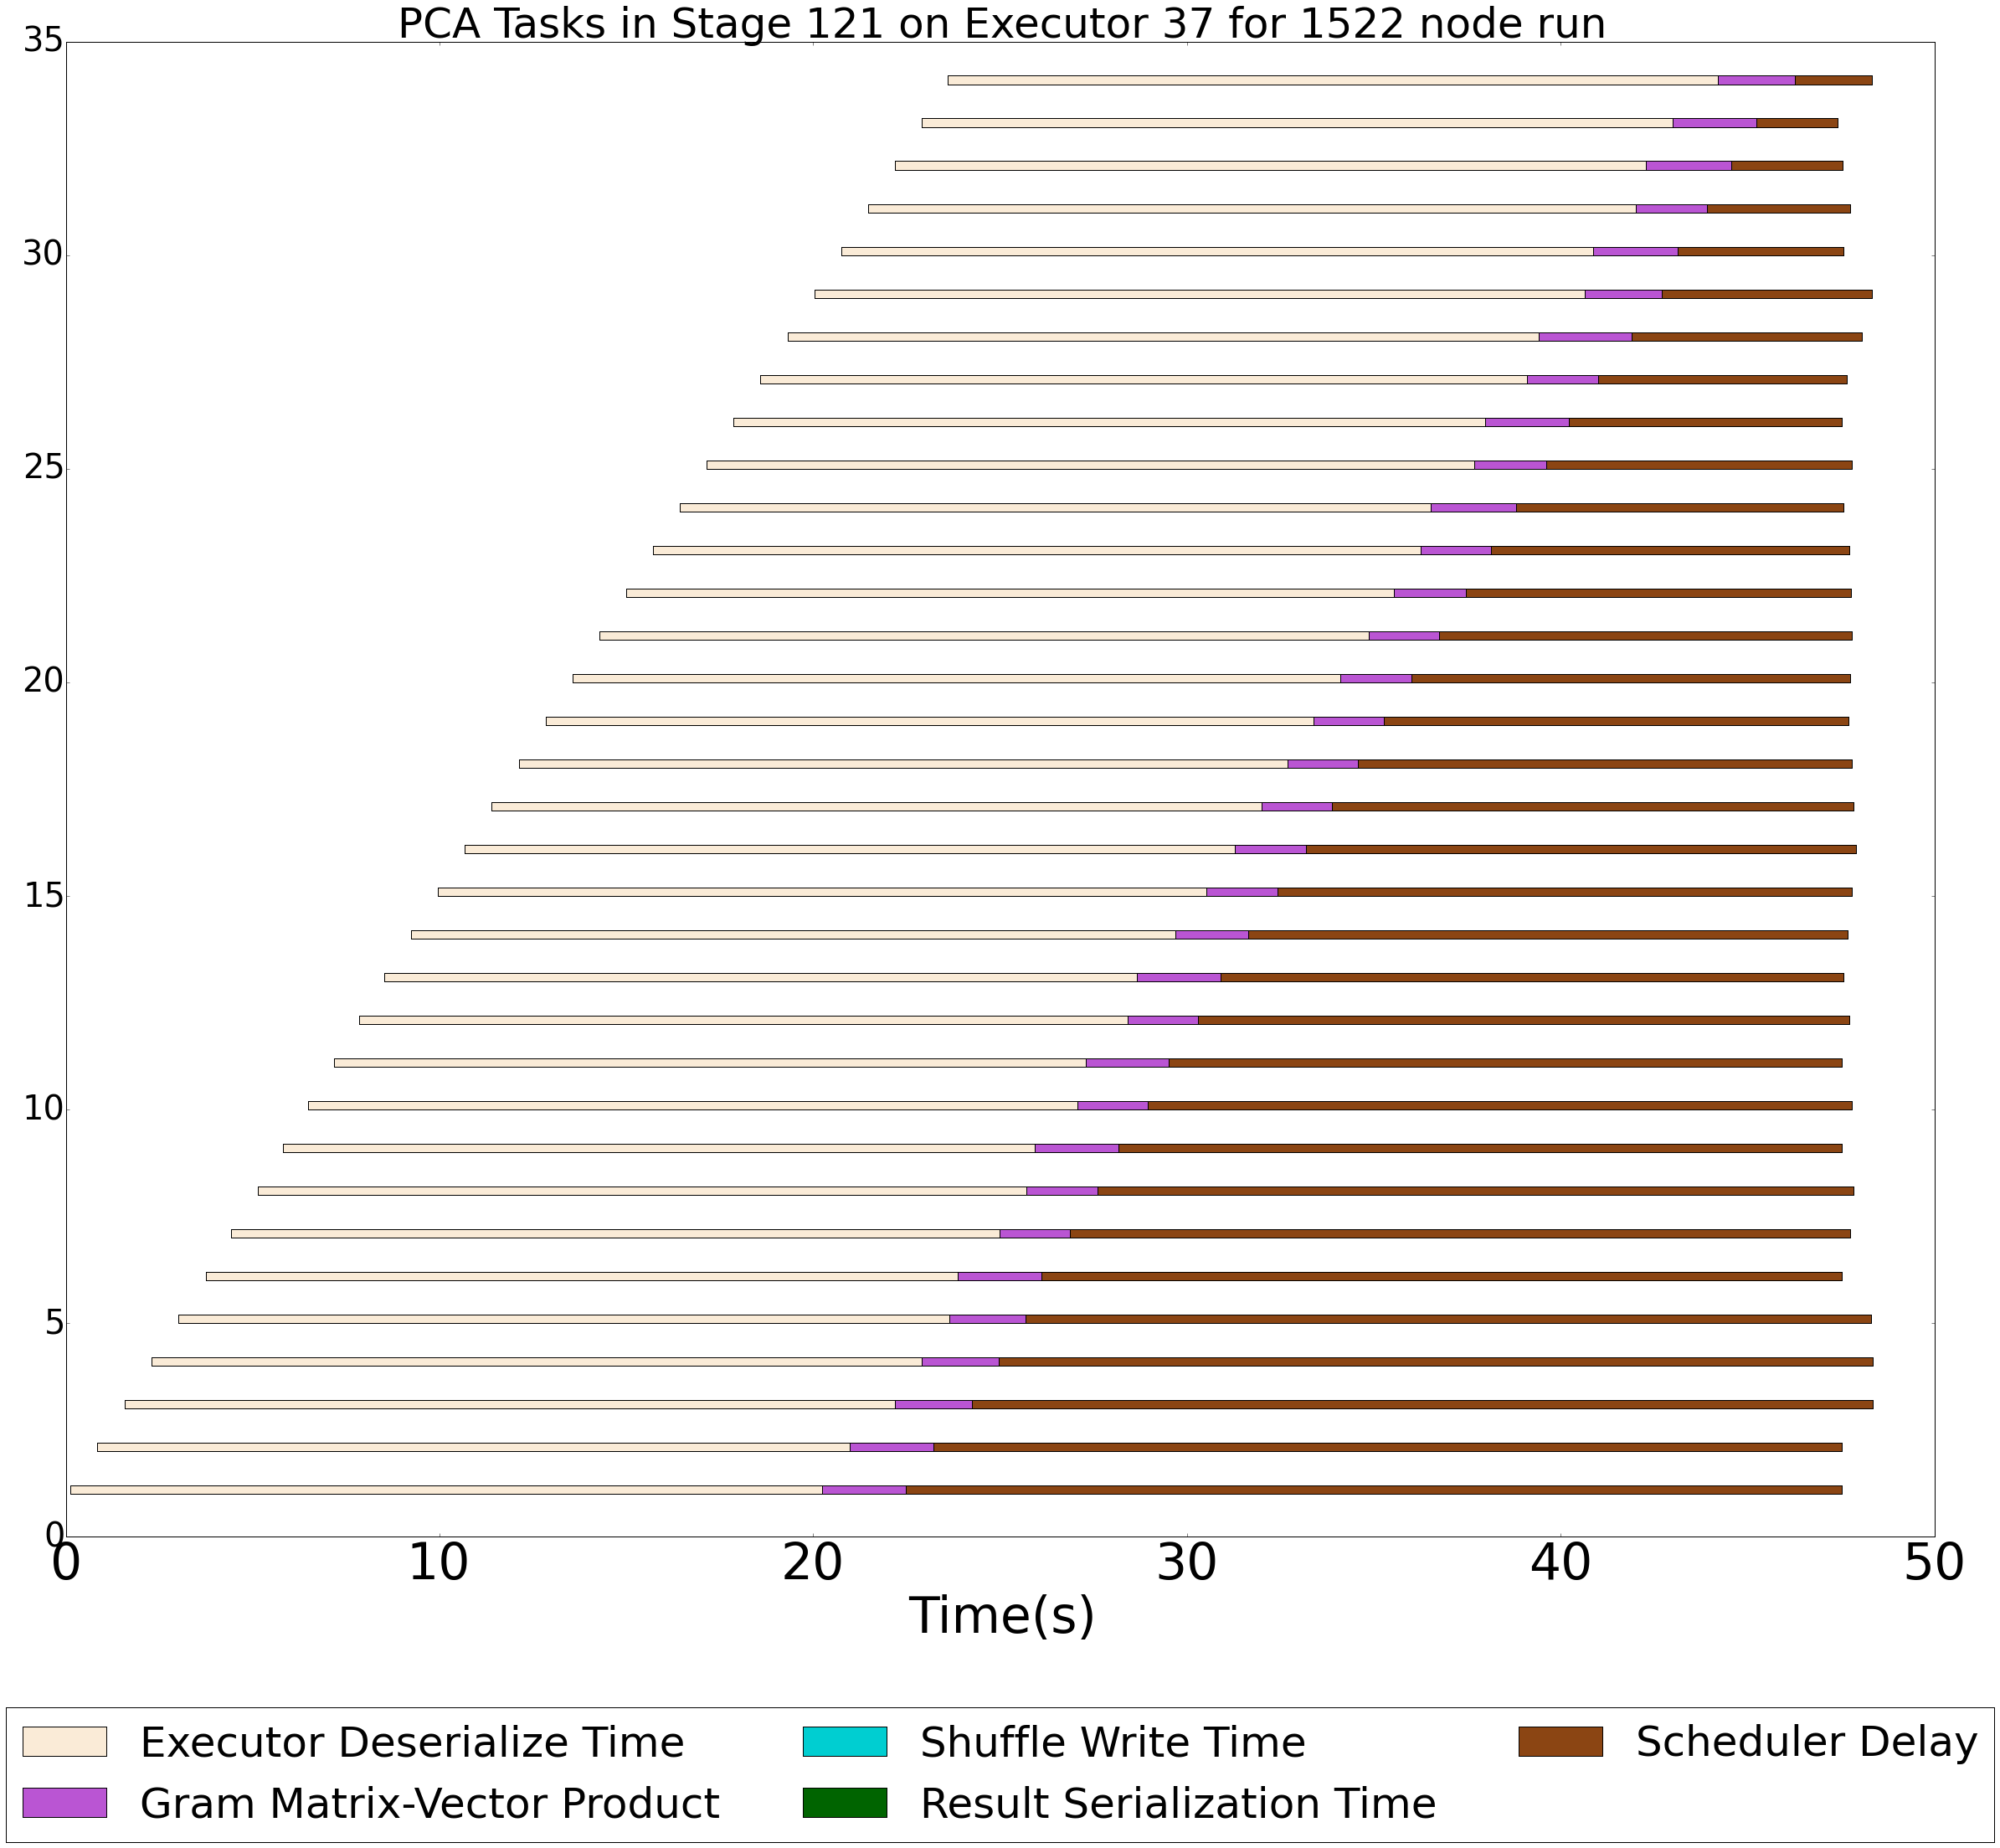
\includegraphics[width=.6\textwidth]{fig/spark_pca_hero_timeline.png}
\caption{A timeline of tasks on a particular node for a multiply Gramian stage during the 1522 node Spark run. }
\label{fig:hero-timeline}
\end{figure}

\begin{figure}[tbhp]
\centering
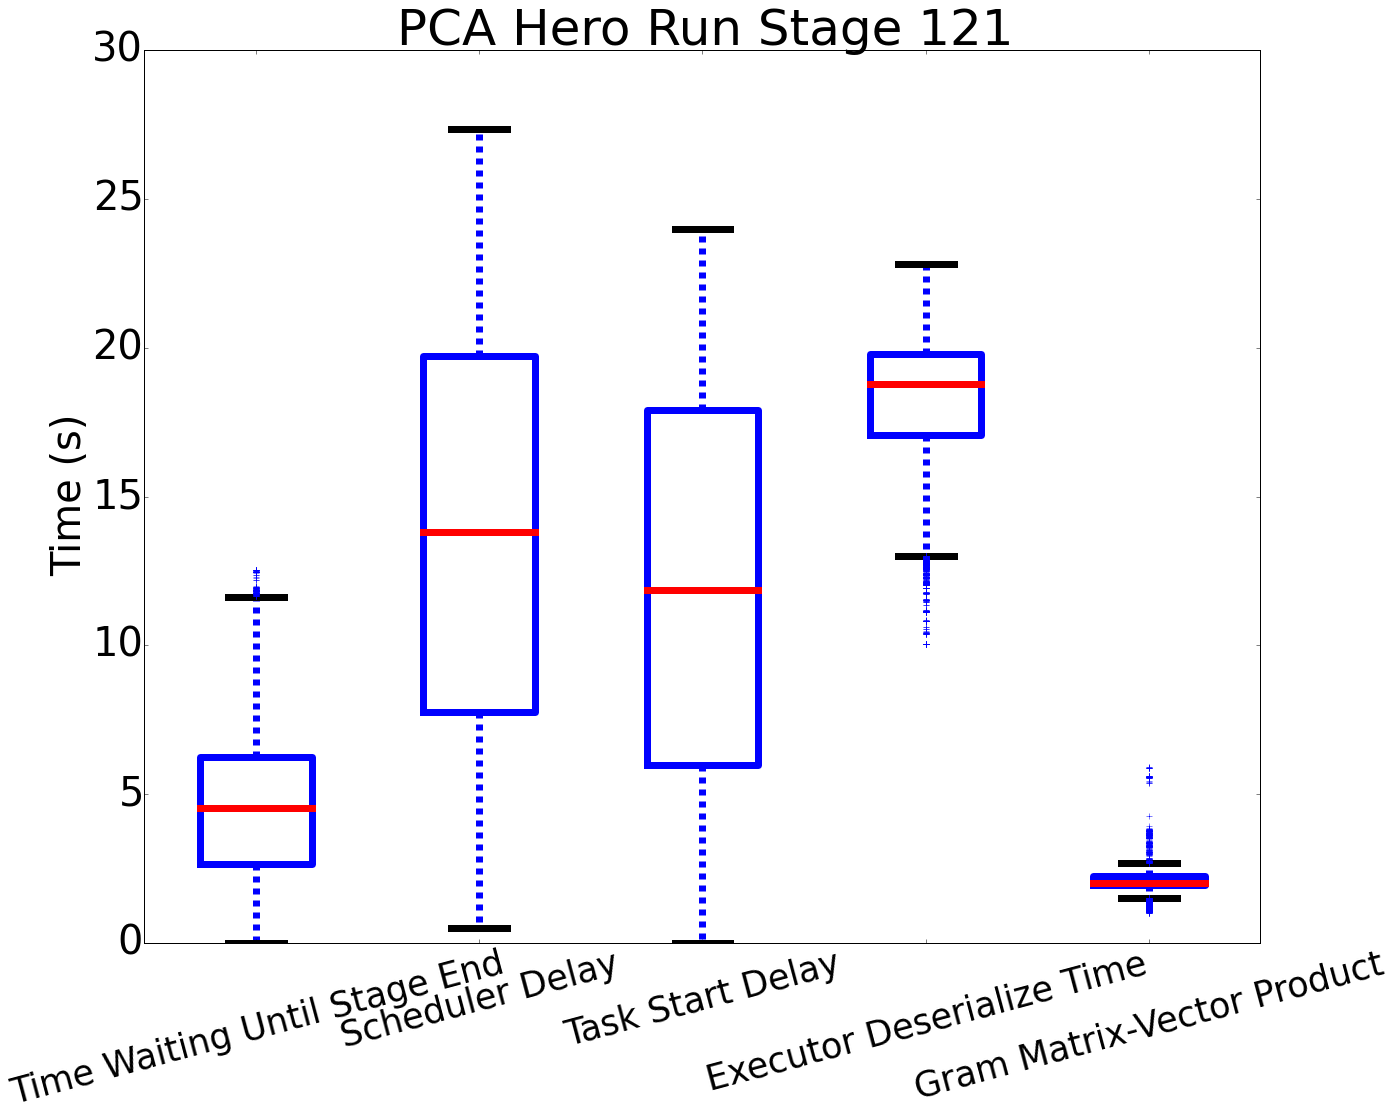
\includegraphics[width=.6\textwidth]{fig/pca_box_and_whiskers.png}
\caption{Distribution of various components of all tasks in a multiply Gramian stage in the Spark PCA hero run. }
\label{fig:whisker}
\end{figure}
\paragraph{Other Significant Spark Overheads.}
Figures \ref{fig:nmfspark} and \ref{fig:sparkpca}, highlight a large block of time spent in Task Overheads. These consist of  shuffle read and write time, task deserialization time (Executor Deserialize Time), and result serialization time.  During our runs on Cori, most of these are insignificant with the exception of Executor Deserialize time, which can be seen in  Figure~\ref{fig:whisker}.  High Executor Deserialize time is usually caused by large tasks that take a long time to unpack. Also, any garbage collection time occuring during the deserialize phase counts toward the deserialize time.

\paragraph{Spark Variability and Stragglers.}
The Time Waiting for Stage to End bucket describes the idle time in which a task has finished, but the next stage has not started, so new tasks have not yet been scheduled. The main cause of this idle time is ``straggler" tasks, tasks that take a longer than average time to finish and thus hold up the next stage from starting. In Figure~\ref{fig:whisker}, we can see there is some variability in multiply Gramian component of tasks, but that is insignificant compared to the Spark overheads: Scheduler and Task Start Delay, as well as Task Deserialization time. These overheads vary anywhere from less than a second to more than 20 seconds. This variation in task behavior leads to some task slots left idle for up to 10 seconds.

The globally-synchronized execution model of Spark creates scaling issues in the presence of stragglers. When a small number of tasks take much longer to complete, many cores end up stuck idling at barriers. At larger scales, we see increases in both the probability of at least one straggler, as well as the number of underutilized cores waiting at barriers.

During initial testing runs of the Spark PCA algorithm, variations in run time as large as 25\% were observed (in our staging runs we had a median run time of 645 seconds, a minium run time of 489 seconds, and a maximum run time of 716 seconds). These variations could not be attributed to any particular spark stage. Sometimes the delay would occur in the Multiply Gramian step, other times in the intial data collect stage. This variability is illustrated in the box and whiskers plot. Spark has a ``speculation" functionality which is aimed at reducing this variability somewhat. However, we found that turning the functionality on had no appreciable effect on improving the run time because the overhead to fetch an RDD from another worker was sufficiently high. This is because requests for RDDs from other workers must wait until the worker finishes its running tasks. This can often result in delays that are as long as the run time of the straggling task.  



\section{Conclusion}
\label{sec:conclusions}
\textcolor{red}{Aditya, Mike, Kristi: I need your input here.}
Major conclusions:
\begin{itemize}
\item{Spark is 2-10x slower for a range of matrix factorization workloads compared to C+MPI implementations. If we remove I/O times from the consideration to purely focus on algorithmic execution, the performance gap widens to 7-25x.}
\item{Spark can be scaled to 1600 nodes on a Cray XC40 system. However, at that scale the overheads associated with scheduling and ??? completely dominate the runtime.}
\item{Given the large performance gap between Spark and C+MPI, it might be wortwhile to investigate integration/interfacing of linear algebra libraries with the Spark runtime. The cost of copying data between runtimes might be worth the performance penalty.}
\item{Efficient I/O is critical for Data Analytics at scale. System architectures in the future will need to be balanced to support data (and hence I/O intensive) workloads.}
\item{}
\item{}
\end{itemize}


\section*{Acknowledgments}
This research used resources of the National Energy Research Scientific
Computing Center, a DOE Office of Science User Facility supported by the Office
of Science of the U.S. Department of Energy under Contract No.
DE-AC02-05CH11231. 

The authors thank Doug Jacobsen, Woo-Sun Yang, Tina Declerck and Rebecca
Hartman-Baker for assistance with the large scale runs at NERSC. Edgar
Solomonik, Penporn Koanantakool and Evangelos Georganas provided helpful comments
and suggestions on tuning the MPI codes. We would like to acknowledge Craig
Tull, Ben Bowen and Michael Wehner for providing scientific data sets used
in the study. We are also grateful to the Daya Bay Collaboration for giving
us access to their experimental data.

This research is partially funded by DARPA Award Number HR0011-12-2-0016, the
Center for Future Architecture Research, a member of STARnet, a Semiconductor
Research Corporation program sponsored by MARCO and DARPA, and ASPIRE Lab
industrial sponsors and affiliates Intel, Google, Hewlett-Packard, Huawei, LGE,
NVIDIA, Oracle, and Samsung.  This work is supported by Cray, Inc., the Defense
Advanced Research Projects Agency XDATA program and DOE Office of Science
grants DOE DE-SC0010200 DE-SC0008700, DE-SC0008699. AD is supported by the
National Science Foundation Graduate Research Fellowship under Grant No. DGE
1106400. Any opinions, findings, conclusions, or recommendations in this paper
are solely those of the authors and does not necessarily reflect the position
or the policy of the sponsors.


\nocite{*}
\bibliographystyle{abbrv}
\bibliography{refs}

%\addtolength{\textheight}{-12cm}   
\end{document}
